\documentclass[manuscript,screen,review,anonymous]{acmart}
\usepackage{tabularx}
\setcopyright{none}
\settopmatter{printacmref=false}
\acmConference{}{}{}
\acmBooktitle{}
\acmDOI{}
\acmISBN{}
\renewcommand{\shortauthors}{Anonymous authors}
\newcommand{\HumT}{\textsc{HumT}}
\newcommand{\Dcrit}{\ensuremath{\overline{D}\geq 3}}
\newcommand{\Fcrit}{\ensuremath{\overline{F}<4}}
\newcommand{\OAcrit}{\ensuremath{\overline{\mathrm{OA}}<4}}
% Generated from frozen screening.csv.
\newcommand{\MHRecall}{25.5\%}
\newcommand{\MHDelta}{+5.5}
\newcommand{\MHAdjusted}{[-2.0, +13.8]}
\newcommand{\MHAP}{0.318}
\newcommand{\EDRecall}{58.3\%}
\newcommand{\EDDelta}{+38.3}
\newcommand{\EDAdjusted}{[-19.8, +80.1]}
\newcommand{\EDAP}{0.109}
\newcommand{\GHRecall}{43.5\%}
\newcommand{\GHDelta}{+23.5}
\newcommand{\GHAdjusted}{[+0.1, +50.5]}
\newcommand{\GHAP}{0.225}

% Additional exploratory paired estimates, percentage points.
\newcommand{\MHWorkRandom}{-8.9 [-15.8, -2.6]}
\newcommand{\MHWorkLength}{+4.7 [-5.3, +14.4]}
\newcommand{\MHWorkMarkers}{+7.4 [-1.2, +19.2]}
\newcommand{\MHFusionDelta}{-1.2 [-7.9, +5.0]}
\newcommand{\EDWorkRandom}{-39.5 [-66.1, +9.0]}
\newcommand{\EDWorkLength}{-30.1 [-71.6, +23.0]}
\newcommand{\EDWorkMarkers}{+13.7 [-9.2, +64.9]}
\newcommand{\EDFusionDelta}{+0.0 [-33.3, +36.4]}
\newcommand{\GHWorkRandom}{-33.1 [-49.2, -17.1]}
\newcommand{\GHWorkLength}{-37.1 [-55.3, -18.8]}
\newcommand{\GHWorkMarkers}{+31.1 [+12.6, +46.8]}
\newcommand{\GHFusionDelta}{-17.4 [-38.5, +0.0]}

% Held-out incremental recall, percentage points.
\newcommand{\MHDConditional}{-2.4 [-6.0, +2.3]}
\newcommand{\MHFConditional}{+1.1 [-8.2, +4.1]}
\newcommand{\MHOAConditional}{+3.0 [-3.9, +8.5]}
\newcommand{\EDDConditional}{+8.3 [-28.6, +33.3]}
\newcommand{\EDFConditional}{+0.0 [-15.0, +7.4]}
\newcommand{\EDOAConditional}{+0.0 [-15.4, +11.8]}
\newcommand{\GHDConditional}{+0.0 [-15.0, +12.0]}
\newcommand{\GHFConditional}{+0.8 [-5.6, +8.7]}
\newcommand{\GHOAConditional}{+0.0 [-9.1, +9.1]}

% Common-queue adversarial-minus-natural recall, exploratory pp.
\newcommand{\MHQueueOAGap}{-17.8 [-34.2, -5.0]}
\newcommand{\GHQueueFitGapH}{+26.1 [+8.6, +44.3]}
\newcommand{\GHQueueFitGapM}{+55.5 [+39.0, +71.1]}
\newcommand{\GHQueueNaturalFitContrast}{+5.4 [-1.3, +13.0]}

% Generated from verified annotation outputs; do not edit values manually.
\newcommand{\IAN}{660}
\newcommand{\IAPositive}{19}
\newcommand{\IAClusters}{13}
\newcommand{\IASlots}{132}
\newcommand{\IAHCaught}{6}
\newcommand{\IAMCaught}{12}
\newcommand{\IAHMissed}{13}
\newcommand{\IAMMissed}{7}
\newcommand{\IAHRecall}{31.6\%}
\newcommand{\IAMRecall}{63.2\%}
\newcommand{\IAHDeltaMarkers}{-31.6}
\newcommand{\IAHDeltaRandom}{+11.6}
\newcommand{\IAHMarkersInterval}{[-66.7, +4.3]}
\newcommand{\IAHRandomInterval}{[-6.7, +30.0]}
\newcommand{\IAAgreement}{97.9\%}
\newcommand{\IAKappa}{0.698}
\newcommand{\IAPositiveAgreement}{70.8\%}
\newcommand{\IABothYes}{17}
\newcommand{\IABothNo}{629}
\newcommand{\IAOnlyFirst}{12}
\newcommand{\IAOnlySecond}{2}
\newcommand{\IADisputes}{14}
\newcommand{\IAInsideD}{15}
\newcommand{\IAOutsideD}{4}

\title{When Tone Scores Allocate Attention: Auditing HumT-Based Review Prioritization}
\author{Anonymous Author(s)}
\begin{document}
\begin{abstract}
Which AI responses receive scrutiny when human review is limited? We audit HumT-based prioritization on 1,490 responses across mental health, education, and general health. Three findings distinguish useful enrichment from justified allocation. First, outperforming random selection need not imply competitiveness with inexpensive alternatives: at 20\% capacity, HumT captures 10 of 23 general-health anthropomorphic-implication cases, compared with 21 for normalized conversational markers. Second, the preferred rule depends on the review criterion; fit and overall-appropriateness comparisons are mixed. Third, aggregate coverage can conceal category-level omissions within the same queue. A separate mental-health assessment tests the unchanged rankings against a contextual reviewworthiness target, while a prompt-group-held-out comparison tests HumT's incremental value beyond lexical features; these estimates remain uncertain. We contribute an exploratory audit of measurement use, linking the target, review budget, comparator and distribution of missed concerns. Review owners should justify these choices together rather than use enrichment alone to select a screen. The study evaluates offline selection against judgments, not experienced harm or subsequent review effectiveness.
\end{abstract}
\keywords{AI evaluation, anthropomorphism, measurement validity, review allocation, algorithmic auditing}
\maketitle

\section{Introduction}
Limited human capacity makes review allocation an explicit decision problem~\cite{okati2021triage}. An inexpensive score could prioritize model outputs without directly measuring the review criterion. Yet its association with human judgments does not establish which cases an allocation rule captures or whether it improves on simpler alternatives.

This distinction matters for anthropomorphic AI language. Expressions of understanding, apparent emotion, conversational familiarity, and first-person reference can make an interaction feel human-like. Such language is not inherently inappropriate. Its interpretation depends on what is expressed and the interactional setting~\cite{devrio2025taxonomy,cheng2025dehumanizing}. A tone score can summarize aspects of this language without establishing whether the response is misleading, fits its domain, or merits escalation. \HumT{} measures human-like language~\cite{cheng2025humt}; its authors do not claim that it is a calibrated probability of harm or a validated human-review policy.

We investigate a proposed downstream use, not a flaw in the metric's original purpose: a model-evaluation team can inspect only a fraction of a response batch. HumT is a plausible candidate for anthropomorphic-language concerns; other targets require separate justification. We evaluate selection against source judgments and a new mental-health assessment follow-up, without establishing workflow adoption, observing subsequent review, or treating non-selection as clearance.

Our central question is: \emph{When review capacity is limited, which concerns does HumT-based prioritization identify, which remain unreviewed, and how does this depend on the criterion and context?} We address three research questions:
\begin{description}
\item[RQ1: Comparative allocation.] At matched review budgets, how does HumT compare with random selection and transparent baselines across source criteria and a separate mental-health reviewworthiness assessment?
\item[RQ2: Incremental value.] Does adding HumT improve recall in a specified marker/length screening model evaluated on held-out prompt groups?
\item[RQ3: Distribution of coverage.] What does aggregate performance omit about review slots and unreviewed concerns across recorded categories within a shared queue?
\end{description}

PERSONA's existing corpus and original judgments were developed for overall-appropriateness prediction. We reuse that resource to study a different decision: which responses enter an exact-capacity review queue. The additions are matched-budget comparisons, held-out incremental screening analysis, shared-queue coverage diagnostics, and new contextual reviewworthiness judgments on the existing mental-health responses. The response corpus is reused; the new judgments are not a new response sample. Appendix~\ref{app:reuse} documents the relationship to the companion work.

Our contribution is an empirical audit distinguishing enrichment, comparative allocation, incremental value, and category coverage. These distinctions organize evidence that a review owner can act on: compare inexpensive alternatives at the same capacity, retain criterion-specific results, and inspect what remains outside the queue. Workload summaries and a worked reporting card make that decision record explicit. The contribution is evaluation practice grounded in this corpus, rather than a new ranking algorithm.

The accountable actor is the evaluation team choosing the target, budget and ranking rule. Its choices allocate scarce opportunities to inspect generated responses. Unnecessary selection consumes reviewer time; an omitted concern loses an opportunity for examination in that pass. Users may bear downstream consequences if problematic responses are later released, although our study does not measure that pathway. These are distinct costs, and affected users need not share the team's concern definition. The natural/adversarial partition is a diagnostic of allocation, not a demographic fairness axis. Our FAccT contribution is to make the evidence needed to justify this evaluation decision inspectable.

\section{Related Work and Conceptual Scope}
\subsection{Human-like language and contextual interpretation}
HumT DumT measures and controls human-like language~\cite{cheng2025humt}. DeVrio et al.'s taxonomy distinguishes linguistic expressions contributing to anthropomorphism, including personal reference and apparent mental states~\cite{devrio2025taxonomy}; it is not a harm scale or a direct mapping to our numerical constructs. Dehumanizing Machines examines interventions and contextual tradeoffs~\cite{cheng2025dehumanizing}. Context dependence motivates this audit rather than constituting its discovery.

FAccT studies of minoritized cues~\cite{basoah2025hunty} and parasocial agency~\cite{maeda2024parasocial} likewise discourage treating anthropomorphism as a uniformly undesirable scalar. We evaluate review selection, not identity perceptions, attachment or longitudinal effects.

AnthroBench evaluates 14 anthropomorphic behaviors in multi-turn interactions and validates their relationship to users' anthropomorphic perceptions~\cite{ibrahim2026anthrobench}. Our endpoint differs: selection against specified review judgments at a fixed capacity, not users' perceptions or multi-turn behavior. Contextual anthropomorphism evaluation itself is not our claimed novelty.

\subsection{From measurement validity to use validity}
Measurement and Fairness emphasizes the relationship between constructs and their operationalization~\cite{jacobs2021measurement}. Evaluation Gaps documents tensions between model-oriented evaluation and application-grounded evaluation~\cite{hutchinson2022gaps}. Applied here, a distinction is necessary between measuring human-like tone, associating tone with a rubric judgment, and establishing useful allocation of human attention. A score may support one of these tasks without supporting the others.

The evaluation target also requires scrutiny. Human ratings operationalize judgments under a rubric and rater population; they do not become objective harm outcomes merely because they are used as labels. Work on representational-harm measurement likewise motivates care about what an observable measure does and does not capture~\cite{chien2024beyond}. We retain separate criteria rather than treating empathy, misleading implication, fit, and holistic appropriateness as interchangeable. Criterion differences may reflect thresholds and prevalence as well as substantive distinctions.

\subsection{Budgeted triage and deferral}
Okati et al. optimize prediction under limited human involvement; Mozannar and Sontag learn when to defer to an expert~\cite{okati2021triage,mozannar2020defer}. OpenL2D/FiFAR benchmarks deferral with synthetic experts and per-batch capacity constraints~\cite{alves2025openl2d}. Capacity-aware routing is not new. Unlike systems modeling expert behavior, we compare rankings against concern judgments without observing subsequent reviewer decisions. Non-selection is not an automated negative judgment. Our contribution is empirical operating points and coverage distributions, not combined human--machine accuracy or a new routing mechanism.

\subsection{Auditing and reporting}
Internal algorithmic auditing and assurance frameworks situate evaluation within broader processes of scoping, evidence gathering, and accountability~\cite{raji2020accountability,lam2024assurance}. Our simulation is not an end-to-end audit. It evaluates one possible selection component and specifies information needed before an organization could responsibly interpret it.

Model cards and datasheets provide precedents for documenting intended uses, evaluation conditions, and data provenance~\cite{mitchell2019modelcards,gebru2021datasheets}. We adapt this documentation orientation to a review-allocation card, including residual unreviewed concerns and a proposed route to challenge a criterion or selection decision. The card is a design proposal, not a validated intervention. The gap addressed is operational: existing tone measurements and appropriateness associations do not directly state how many criterion-defined cases enter a fixed-capacity queue relative to simple alternatives.

\section{Corpus, Provenance, and Criteria}
\subsection{Existing corpus and annotation}
The final analytical corpus contains 1,490 English, single-turn responses in 499 domain-scoped prompt clusters: 660 responses and 220 clusters for mental health; 415 and 139 for education; and 415 and 140 for general health. Responses derive from three model endpoints and natural and adversarial prompt sets. Prompt sets are unmatched across conditions. Domain, source material, rater population, and score distributions vary together, so domain comparisons do not isolate a causal context effect.

Each response has a recorded automated score $H$ and five ratings for each of empathic appropriateness ($E$), misleading anthropomorphic implication ($D$), domain fit ($F$), and overall appropriateness (OA). Higher $D$ indicates greater concern; higher $F$ and OA indicate more favorable judgments. We reconstruct every stored construct mean from the released ratings. All recorded HumT values are finite; HumT is not treated as a probability.

The source study's final documentation describes two non-overlapping rater groups. Group A comprises three domain-specific pools of five raters each and supplies OA. A separate five-person Group B supplies $E/D/F$ across domains and includes authors and research interns familiar with the framework. These are operational targets under the source rubric, not independent ground truth for anthropomorphic harm. OA provides a separate-rater, different-construct endpoint, not an independent replication of the $D$ judgments. Domain-relevant backgrounds are documented as mental-health/psychology training, medical training, and teaching experience; professional licenses are not inferred. Phase labels distinguish rating tasks, not shared personnel; the final application note states that the same-rater fallback was not used.

\paragraph{Agreement and cutoff stability.}
We reconstruct two-way absolute-agreement ICC point estimates and retain the source Krippendorff ordinal alpha (Table~\ref{tab:reliability}). For $D$, average-rating ICC(A,5) is 0.959, 0.963 and 0.942 across the three domains, versus ordinal alpha of 0.840, 0.843 and 0.446. Reliability of averaged ratings is not construct validity or independence. Source reliability intervals resample responses, unlike our prompt-cluster screening intervals. Cutoff proximity and mean-versus-majority disagreement are reported for all criteria in Appendix~\ref{app:labels}; 108 mental-health means lie exactly at $D=3$.

\subsection{Input and reuse audit}
Every stored mean is reconstructed from the source ratings, and source scores and judgments remain unchanged. Mental-health HumT values are embedded in the records; transfer-domain values are joined from exports. Some export strings differ from annotated text, so the imported score and lexical baselines may reflect different representations. Appendix~\ref{app:sensitivity} reports the exact join audit and fixed-capacity checks; historical scorer calls cannot be authenticated from the exports alone.

The corpus is not a deployment sample. Its mixture weights, condition frequencies, and model endpoints do not estimate real organizational demand. Most prompts have three responses; there are incomplete model sets in education and general health. Complete-set model comparisons retain 220, 138, and 136 prompt clusters, respectively. We never infer model-family rankings from these three endpoints.

\subsection{Concern criteria}
\paragraph{PERSONA as an evaluation profile.}
PERSONA supplies contextual $E/D/F$ judgments and separately elicited OA, not a scalar replacement for HumT or a chatbot-persona prompt. These judgments define endpoints, not test-time inputs to fixed screens. Human assessment before selection would incur annotation costs; ranking by the same labels used to evaluate success would be an oracle.

Our candidate primary trigger is \Dcrit{}, where the bar denotes the mean of five ratings. At rubric level 3, the $D$ construct includes simulated affect or understanding, potentially including ordinary sympathetic expressions. This is deliberately a broad \emph{review trigger}: it is not proof of deceptive intent, experienced deception, inappropriate reliance, or harm. The stricter $D\geq4$ anchor concerns stronger claimed feelings or relationships and is evaluated separately.

Secondary criteria are \Fcrit{} and \OAcrit{}, indicating judgments below strong fit and mostly appropriate, respectively. Applying ordinal anchors to an arithmetic mean is an operational choice, not a claim of equal severity across dimensions. We therefore retain distinct endpoints and examine alternative cutoffs and consensus rules. $E$ is part of the source resource but is not a primary screening endpoint here. Human judgments are not test-time screening features. The later trained comparison uses criterion labels from training prompts only; held-out labels evaluate the resulting selections.

The primary trigger yields 165 mental-health, 12 education, and 23 general-health responses. The corresponding concern-bearing prompt counts are 99, seven, and 15. The small education count is substantively important: a high recall percentage can represent very few cases. Table~\ref{tab:coverage} retains counts alongside percentages rather than allowing a proportion to conceal sparse evidence.

The marker baseline shares cues with broad $D$, but cannot enforce its exclusions for functional first-person grammar, quotations or others' claims. It tests recovery from surface cues, not a competing ground truth. Fit and separately rated OA provide complementary endpoints, not substitutes selected for a preferred policy ordering.

\subsection{New mental-health assessment follow-up}\label{sec:assessment}
The follow-up covers the complete \IAN{}-response mental-health batch, not a sample selected for policy success. Assessors R1, R2 and R3 were outside the original author/rater team. R1 and R2 each supplied a full-corpus stream; R3 independently assessed only their \IADisputes{} binary disagreements without seeing the preceding labels. Packets withheld policy scores and prior judgments. Assessors were instructed to work independently and not use AI-generated judgments. R3's selective coverage is resolution of disagreements, not a third complete rating stream.

The task is to identify an anthropomorphic implication that warrants human review in context, not any human-like wording or general safety problem. Ratings are 0 (no target concern), 1 (human-like language without sufficient reason for review), 2 (plausible misleading or unsupported implication), 3 (clear or substantial implication warranting priority review), or U (insufficient information). Ratings 2/3 define the binary target; 0/1 do not. Assessors are asked to consider attribution, quoted speech, and the full prompt--response pair, and supply a supporting passage and contextual rationale for a flag. Ordinary sympathy and first-person pronouns are explicitly insufficient on their own. Priority review is not evidence that harm occurred.

R1 used capability note v1.0; R2 and R3 used v1.1. The latter distinguishes verified information, fixed study assumptions, and unknown capabilities, including that missing tool logs do not prove the absence of external actions. Capability-dependent judgments remain conditional on those assumptions. Because assessor and note version vary together, observed agreement is not same-instruction reliability and cannot isolate a version effect. No records are excluded to improve agreement. We preserve R1/R2 binary agreements and resolve disagreements by two definite votes after R3's assessment, retaining unresolved cases if no such majority exists. All current cases resolve; this does not constitute three-assessor coverage of the whole corpus.

The computational specification was recorded after inspecting these judgments and point estimates. This is an exploratory amendment, not preregistration. We evaluate the original HumT, normalized-marker and word-length rankings, original tie rule, and exact capacities without retraining on the new labels. Random performance is an analytical matched-budget expectation. The supplied package's alternative lexical queues are kept separate rather than silently replacing the original baselines (Appendix~\ref{app:assessment}). Rater-specific, union/intersection, and rating-3 targets retain disagreements as sensitivity evidence. The original primary family, trained analysis and CHI results are unchanged.

\section{Screening Evaluation}
\subsection{Decision and policies}
\paragraph{Two distinct tools.}
The response-generating chatbot and the review-allocation screen have different design assumptions. We vary the latter's ranking policy and capacity on fixed outputs, not the former's persona, expressive constraints, memory, or service role. The corpus does not implement a matched scripted-versus-open-ended comparison; model and prompt-condition labels cannot substitute for that treatment. Capability-dependent judgments in the follow-up are conditional on the supplied notes, not verified deployment configurations. Thus, the reported ordering applies to these response batches and criteria, not to all chatbot designs.

The accountable actor in the proposed workflow is an evaluator responsible for a defined response batch. The review unit is a prompt--response pair, and selection creates an opportunity for subsequent manual assessment rather than an automatic adverse action. We do not observe review findings, escalation, or remediation. Non-selection means that an item has not entered this review queue; it does not mean cleared, safe, or appropriate.

For a batch of $n$ responses and budget fraction $b$, capacity is $k=\lfloor nb\rfloor$. We evaluate $b\in\{.05,.10,.20,.30\}$. The already-explored 20\% budget is a reference operating point, not a retrospectively optimized optimum. Primary analyses use separate domain batches; pooled analyses are secondary.

Three fixed policies rank scores in descending order: \textbf{high-H} uses recorded HumT; \textbf{length} uses regex word-token count; and \textbf{markers} uses the fraction of tokens in a fixed first/second-person and conversational-marker dictionary (Appendix~\ref{app:implementation}). The marker score is a transparent lexical comparator, not an independently validated anthropomorphism metric. These rules require no task-specific human training labels, unlike the separately evaluated logistic screens below.

A post-review amendment adds one untuned \textbf{rank-fusion} policy: the equal-weight mean of within-batch midrank percentiles for HumT and markers, selected at the same exact capacity. It uses no labels or fitted weights; ranks are recomputed within each bootstrap batch. Selected-set intersections describe complementary cases, while the larger union is not counted as a same-budget policy. This tests one transparent combination, not the best possible trained screen or conditional independence of the two scores.

Uniform random selection uses the same exact $k$. We compute its expectation analytically, avoiding comparison against one unusually favorable or unfavorable draw. For pooled analyses, an additional stratified random policy allocates slots proportionally by domain using largest-remainder rounding. Deterministic seeded hashes of stable response identifiers resolve ties without exceeding capacity. A 100-seed analysis examines sensitivity to tie resolution. Missing or nonfinite policy scores are rejected rather than silently excluded.

\subsection{Held-out trained comparison and conditional lift}
A second post-review amendment tests the added value of HumT with a transparent trained comparator. For each domain and criterion, the reduced model is L2-regularized logistic regression on marker fraction and $\log(1+\mathrm{length})$; the extended model adds recorded HumT. This model isolates the question of adding one feature to an inspectable screen, not competitiveness with the strongest available evaluator. We make no comparison claim against semantic judges or modern automated review systems generally. Both models use fixed $C=1$, an intercept, LBFGS, and no class weighting or tuning; standardization is fitted on training data only. Their scores rank the source criterion rather than estimate calibrated harm probabilities.

We partition prompt groups into five folds using a seeded, label-independent permutation. Each held-out fold is a separate review batch; all responses to a prompt remain together. Each model trains on the other four folds. We re-evaluate all fixed policies, fusion, and analytical random selection in these same held-out batches. Counts are summed before calculating recall or precision; scores from different fitted models are never pooled into a common ranking. At the 20\% reference fraction, flooring each batch's quota yields 130 total mental-health slots and 80 in each other domain, rather than the original full-batch capacities of 132 and 83. Comparisons therefore use the new matched-batch table, not the original capacities.

We define \emph{conditional lift} operationally as the absolute recall difference
\begin{equation}
\Delta R_{H\mid M,L}=R_{\mathrm{LR}(M,\log(1+L),H)}-R_{\mathrm{LR}(M,\log(1+L))}.
\end{equation}
It tests an incremental contribution within this specified model and workflow, not a causal effect, conditional independence, or all possible uses of HumT. Training uses existing human labels and is not label-free: each mental-health fit uses 528 labeled responses, while transfer-domain counts vary with fold size (Appendix~\ref{app:complete}). Held-out labels are never used to fit their own model. These historical labels are reused across fits; annotation acquisition costs are not estimated, nor are fit-level counts summed as separate purchases.

At the reference fraction we use 2,000 paired prompt-cluster bootstrap draws within the original fold strata, retaining a sampled prompt's original fold. We refit both scalers and models on every draw, re-rank every resampled held-out batch at its exact quota, and use common draws across policies and criteria. A single-class training sample produces an explicitly recorded constant-prevalence score; undefined recall remains undefined. Intervals are exploratory pointwise percentile intervals conditional on this partition, empirical judgments, and prompt distribution. Ten additional pre-specified partitions assess split sensitivity, not independent replication or an opportunity to choose the best seed. Other budgets receive descriptive point estimates.

\subsection{Outcomes and workload}
Let $P$ be the number of responses meeting a criterion and $T$ the number selected that meet it. Recall is $T/P$, precision is $T/k$, and the number of unreviewed concern cases is $P-T$. Concern prevalence among unselected responses is $(P-T)/(n-k)$. Under uniform random selection, expected $T=kP/n$ and expected recall is $k/n$ when $P>0$. Appendix~\ref{app:transfer} retains capacity ceilings and prevalence-relative lift as contextual quantities, not additional independent outcomes.

We also report average precision (AP) and ROC-AUC for ranked policies, with class prevalence. AP uses recall-increment-weighted precision at tied-score block boundaries, not trapezoidal interpolation. Both implementations were independently checked against scikit-learn~\cite{pedregosa2011scikit}. AP complements ROC-AUC when concern prevalence is low~\cite{saito2015precision}; neither makes the human criterion a validated harm outcome.

For a target recall $r$, retrospective workload is the shortest ranking prefix containing at least $\lceil rP\rceil$ concern cases, divided by $n$. We retain the originally specified 50\%, 80\%, 90\%, and 100\% targets; 80\% is a descriptive reference, not a justified service requirement. For random ordering, expected prefix length is $\lceil rP\rceil(n+1)/(P+1)$. These label-informed summaries are not deployable stopping rules or labor-cost estimates.

\subsection{Uncertainty and analysis status}
We use 2,000 paired prompt-cluster bootstrap replicates. All responses for a sampled prompt remain together, and the same resamples support comparisons across policies and criteria. Each replicate re-ranks its resampled batch at the specified capacity. Repeated copies of a cluster receive occurrence-specific tie keys. Pooled resampling is stratified by domain. Thus, intervals characterize a resampled-batch allocation procedure, not application of a previously learned fixed threshold.

Most intervals are exploratory pointwise 95\% percentile intervals. The specified primary comparison family contains three domain-specific high-H minus random recall differences for \Dcrit{} at 20\%, using Bonferroni-adjusted 98.3333\% percentile intervals. This nominal adjustment addresses that family, not all sensitivity analyses. Fewer than ten concern-bearing or nonconcern-bearing prompts triggers a sparse-evidence flag. Recall and AP are undefined without positive cases; AUC requires both classes. We report finite replicate counts rather than substituting zero for undefined values.

Earlier exploration covered alternative OA/$D$/$F$ cutoffs, top-20\% selection, ranking summaries, overlaps and model means. Subsequent amendments added fusion, cutoff/text checks, workload contrasts, trained screens and common-queue analysis. Each specification preceded its computation but followed inspection of earlier findings; none is preregistration of unseen evidence. These additions preserve the original primary family and use exploratory pointwise intervals. Mental health receives emphasis for its larger sample, not as a replacement primary endpoint. Bootstrap intervals condition on supplied judgments; rater-rule sensitivity addresses separate uncertainty. Intervals crossing zero establish neither equivalence nor absence of useful HumT information.

\subsection{Common-queue category coverage}
A third exploratory amendment ranks each domain once at 20\%, then projects selections onto condition, model and scenario categories without reranking or reserving category quotas. All three criteria and five fixed policies are retained. Category counts include slots, concerns, recall and residual cases; zero-concern recall is undefined. Random expected slots are $kn_g/n$ and caught cases $kP_g/n$, not separately floored quotas. Each of 2,000 paired domain-level prompt resamples re-ranks before projection, supporting pointwise category, group-minus-complement and within-group policy contrasts. Condition was specified as the main reporting partition before this run; complete model/scenario results and sparse flags remain available. These unmatched-set comparisons are descriptive, not causal or demographic-fairness estimates.

\section{Results}
\subsection{RQ1: Comparative allocation at matched capacity}
Table~\ref{tab:coverage} shows high-H coverage at 20\%. For \Dcrit{}, the policy selects 42 of 165 mental-health cases, seven of 12 education cases, and ten of 23 general-health cases. Uniform random selection would capture 33, 2.4, and 4.6 cases in expectation. The corresponding HumT precision values are 31.8\%, 8.4\%, and 12.0\%. Enrichment therefore does not imply that most selected responses meet the criterion, especially when the criterion is rare.
\begin{table}[t]
\centering\small
\caption{High-H selection at 20\% capacity. Precision and recall are percentages. $P$ is the number of criterion cases. These are exploratory pointwise intervals, not simultaneous comparisons; education $D$ and general-health OA each have only seven concern-bearing prompts.}
\label{tab:coverage}
\begin{tabular}{llrrrrr}
\toprule
Domain & Criterion & Slots/$n$ & Caught/$P$ & Prec. & Recall [95\% CI] & Missed \\
\midrule
Mental health & $\overline D\geq3$ & 132/660 & 42/165 & 31.8 & 25.5 [19.2, 32.1] & 123 \\
 & $\overline F<4$ & 132/660 & 18/95 & 13.6 & 18.9 [12.2, 27.6] & 77 \\
 & $\overline{\mathrm{OA}}<4$ & 132/660 & 31/133 & 23.5 & 23.3 [17.6, 30.6] & 102 \\
Education & $\overline D\geq3$ & 83/415 & 7/12 & 8.4 & 58.3 [16.7, 90.9] & 5 \\
 & $\overline F<4$ & 83/415 & 10/25 & 12.0 & 40.0 [18.8, 60.0] & 15 \\
 & $\overline{\mathrm{OA}}<4$ & 83/415 & 9/18 & 10.8 & 50.0 [23.5, 73.7] & 9 \\
General health & $\overline D\geq3$ & 83/415 & 10/23 & 12.0 & 43.5 [24.0, 65.2] & 13 \\
 & $\overline F<4$ & 83/415 & 25/120 & 30.1 & 20.8 [13.6, 27.2] & 95 \\
 & $\overline{\mathrm{OA}}<4$ & 83/415 & 3/9 & 3.6 & 33.3 [0.0, 70.1] & 6 \\
\bottomrule
\end{tabular}
\end{table}


In mental health, even perfect selection into 132 slots cannot recover all 165 broad-$D$ cases. This capacity constraint does not explain all omissions: HumT captures 42 cases and leaves 123 unreviewed. Both the available capacity and the ranking must therefore be considered.

The primary-family recall improvements over random are \MHDelta{}, \EDDelta{}, and \GHDelta{} percentage points, with adjusted intervals \MHAdjusted{}, \EDAdjusted{}, and \GHAdjusted{}, respectively. The general-health lower endpoint is very close to zero, and its interpretation depends on the percentile procedure and finite bootstrap resolution. The results do not establish robust superiority across domains or thresholds. Education's \Dcrit{} estimate rests on only seven concern-bearing prompts.

Coverage also depends on the criterion. Mental-health domain-fit recall is 18.9\%, slightly below the random expectation, while general-health fit recall is 20.8\%. For education, high-H recovers ten of 25 fit concerns and nine of 18 OA concerns. The general-health OA estimate of 33.3\% represents three of nine cases across seven concern-bearing prompts and has a wide interval. A case outside one criterion may still satisfy another; neither criterion membership nor non-membership establishes general safety.

Figure~\ref{fig:paired} summarizes all nine paired HumT--marker comparisons alongside the trained incremental comparison. The panels use different, explicitly labeled batch definitions; neither substitutes for the adjusted primary family. Appendix~\ref{app:transfer} retains all domain budget curves.
\begin{figure}[t]
\centering
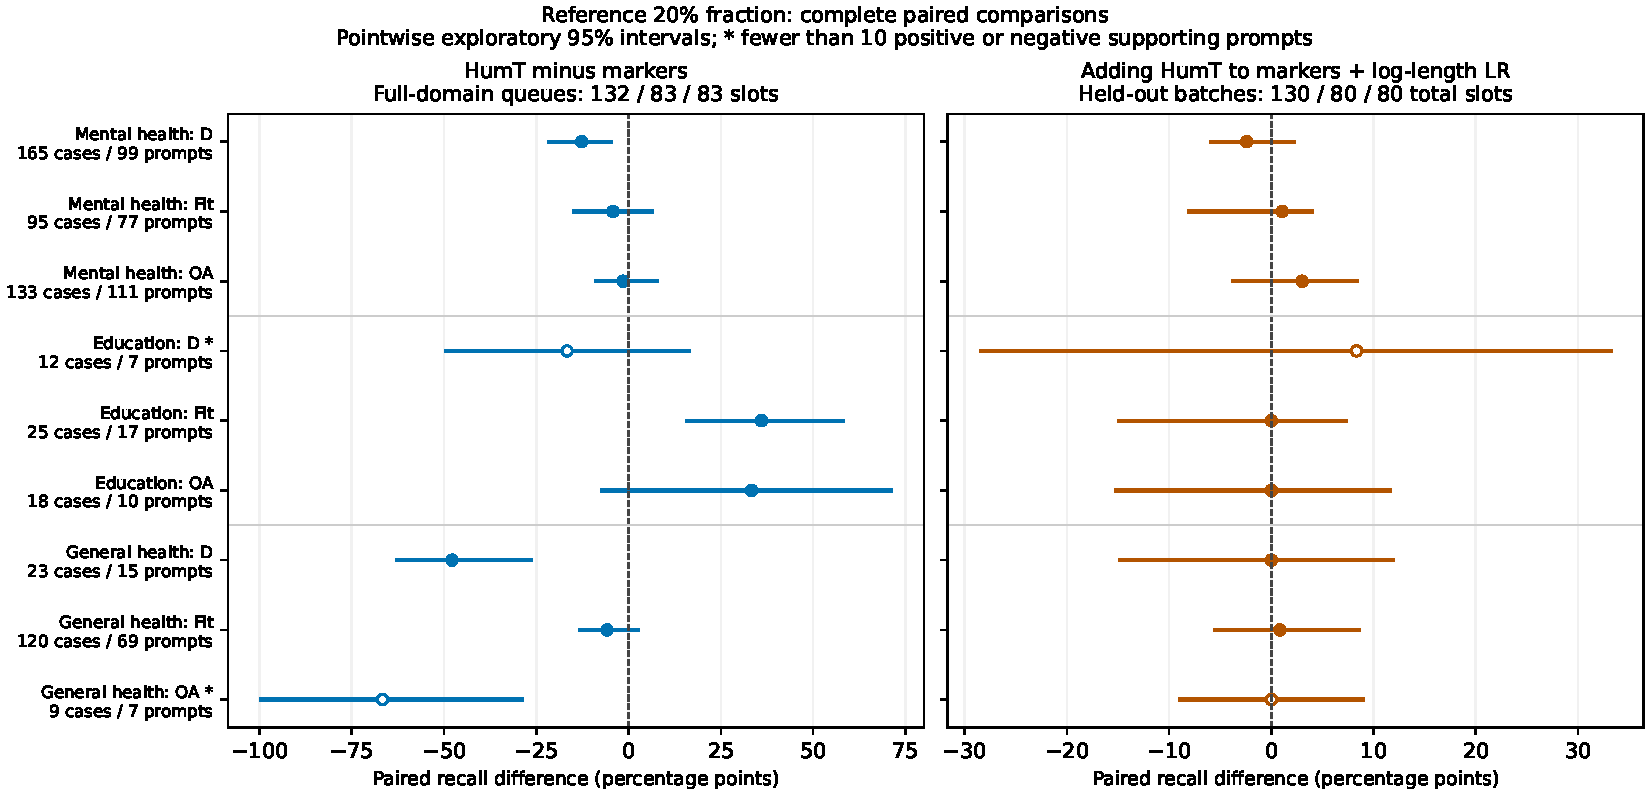
\includegraphics[width=\linewidth]{figures/paired_summary.pdf}
\caption{Complete paired recall contrasts at the 20\% reference fraction. Left: HumT minus markers in original full-domain queues. Right: adding HumT to the marker/log-length logistic screen in common held-out batches, with refitted uncertainty. Positive values favor HumT or its addition. Intervals are exploratory pointwise 95\%, not simultaneous; hollow points mark sparse support. Counts refer to criterion cases and concern-bearing prompts.}
\Description{Two forest plots show all domain and criterion differences. The left panel shows mixed criterion-dependent comparisons; all nine intervals in the trained incremental panel cross zero. Every point has its own paired uncertainty interval and supporting counts.}
\label{fig:paired}
\end{figure}

\paragraph{Transparent alternatives.}
Table~\ref{tab:baselines} compares policies for the primary trigger. The marker policy selects 63 mental-health, nine education, and 21 general-health concern cases at the same capacities as HumT. HumT minus marker recall is -12.7 percentage points in mental health and -47.8 points in general health; their paired pointwise intervals exclude zero. The education difference is -16.7 points but uncertain. Length performs better than HumT for mental-health $D$ coverage and worse in the other two domains; those comparisons are less conclusive.
\begin{table}[t]
\centering\small
\caption{Observable baselines at 20\% capacity for $\overline D\geq3$. Recall is a percentage; paired differences and their exploratory pointwise 95\% intervals are percentage points. Education is sparse.}
\label{tab:baselines}
\begin{tabular}{llrrr}
\toprule
Domain & Comparator & Caught/$P$ & Recall & HumT minus comparator \\
\midrule
Mental health & Length & 54/165 & 32.7 & -7.3 [-14.8, +1.8] \\
 & Markers & 63/165 & 38.2 & -12.7 [-21.9, -4.3] \\
Education & Length & 3/12 & 25.0 & +33.3 [-11.1, +75.0] \\
 & Markers & 9/12 & 75.0 & -16.7 [-50.0, +16.7] \\
General health & Length & 5/23 & 21.7 & +21.7 [+0.0, +47.1] \\
 & Markers & 21/23 & 91.3 & -47.8 [-63.2, -25.9] \\
\bottomrule
\end{tabular}
\end{table}


This is not evidence that marker counting is a universal safety screen. Pronouns and expressions such as sympathy overlap with cues in the broad $D$ rubric. The result shows that an inexpensive observable comparator can recover these particular labels more effectively; it does not show that removing its markers improves an interaction. Ranking-level summaries tell a consistent but distinct story. HumT AP for \Dcrit{} is \MHAP{}, \EDAP{}, and \GHAP{} against prevalences of 25.0\%, 2.9\%, and 5.5\%. Marker AP is 0.465, 0.126, and 0.395, respectively. These values should be read within each criterion and population, not as prevalence-free universal rankings.

The full fit/OA comparison is mixed, not a general reversal of the broad-$D$ result. In mental health, HumT selects 18/95 fit and 31/133 OA cases versus markers' 22/95 and 33/133; both paired recall-difference intervals include zero. In education it selects 10/25 fit and 9/18 OA cases versus 1/25 and 3/18. The education fit-recall difference is +36.0 percentage points (exploratory 95\% interval +15.4 to +58.6); the OA difference is +33.3 points (-7.7 to +71.4). In general health, HumT selects 25/120 fit and 3/9 OA cases versus markers' 32/120 and 9/9: differences are -5.8 points (-13.6 to +2.9) and -66.7 points (-100.0 to -28.5). The latter rests on only seven concern-bearing prompts. Appendix~\ref{app:complete} reports every policy--criterion cell, including length, fusion, and random. These pointwise exploratory findings do not establish universal fit/OA superiority or precise performance on rare concerns.

\subsection{RQ1 follow-up: Contextual reviewworthiness}\label{sec:assessmentresults}
Before resolution, R1 and R2 agree on \IABothYes{} positive and \IABothNo{} negative cases, with \IAOnlyFirst{} R1-only and \IAOnlySecond{} R2-only flags. Binary agreement is \IAAgreement{}, Cohen's $\kappa=\IAKappa{}$, and positive agreement is \IAPositiveAgreement{}. The high raw agreement is dominated by negative cases; neither it nor kappa validates the criterion. R3's disagreement assessments yield \IAPositive{} resolved positives in \IAClusters{} prompt clusters, with no unresolved labels. We do not calculate full-corpus three-rater reliability from selective third assessment.

Table~\ref{tab:annotation_coverage} evaluates the original queues at \IASlots{} slots. HumT captures \IAHCaught{}/\IAPositive{} (\IAHRecall{}) and leaves \IAHMissed{} target cases unreviewed; normalized markers capture \IAMCaught{}/\IAPositive{} (\IAMRecall{}) and leave \IAMMissed{}. The ranking is therefore not evaluated solely against the original broad trigger. However, a secondary 2,000-draw paired prompt-cluster bootstrap, re-ranking each resampled batch at 20\%, gives a HumT--marker recall difference of \IAHDeltaMarkers{} percentage points, with exploratory 95\% interval \IAHMarkersInterval{}. HumT minus expected random is \IAHDeltaRandom{} points, interval \IAHRandomInterval{}. Both intervals include zero. These describe hypothetical batches from the empirical prompt distribution, not uncertainty in the exact corpus counts or in the human judgments; all 2,000 draws are defined.
\begin{table}[t]
\centering\small
\caption{Mental-health assessment follow-up: original frozen policies at 132/660 slots against the resolved target ($P=19$, 13 concern-bearing prompts). Recall and precision are percentages. These are exact corpus counts conditional on mixed-version judgments; random counts are analytical expectations. Paired hypothetical-batch intervals are reported in the text, not inferred from the point ordering.}
\label{tab:annotation_coverage}
\begin{tabular}{lrrrr}
\toprule
Policy & Caught/$P$ & Recall & Precision & Missed \\
\midrule
HumT & 6/19 & 31.6 & 4.5 & 13 \\
Normalized markers & 12/19 & 63.2 & 9.1 & 7 \\
Word length & 4/19 & 21.1 & 3.0 & 15 \\
Random (expected) & 3.8/19 & 20.0 & 2.9 & 15.2 \\
\bottomrule
\end{tabular}
\end{table}


The marker policy also captures more flagged cases in each assessor's own labels, the union/intersection targets, and each assessor's rating-3 target (Appendix~\ref{app:assessment}). This consistent point ordering is not seven independent replications: the targets share responses, judgments and queues. The new labels overlap with, but do not simply refine, the source trigger: \IAInsideD{} of \IAPositive{} positives satisfy broad $D$, while \IAOutsideD{} do not. The follow-up therefore extends the observed comparison to an explicitly contextual target but establishes neither general marker superiority nor an externally validated definition of harm. Its limited positive support constrains extrapolation beyond this batch.

\subsection{RQ2: Incremental benefit beyond lexical features}
\paragraph{Different cases are not a same-budget improvement.}
At the mental-health reference budget, HumT and markers share 22 broad-$D$ cases; HumT selects 20 additional cases that markers miss, while markers select 41 that HumT misses. Their union would require 221 review slots rather than 132, so it is not a fair same-budget alternative. Equal-weight rank fusion selects 61 cases versus markers' 63, a recall difference of \MHFusionDelta{} percentage points (exploratory 95\% interval). For fit and OA it selects 25 and 39 cases versus markers' 22 and 33, but both paired difference intervals include zero.

In education, HumT contributes one broad-$D$ case outside markers' set; in general health it contributes none at this budget. Fusion captures nine and 17 broad-$D$ cases, versus markers' nine and 21. Table~\ref{tab:complementarity} reports all criteria and paired intervals. These overlaps establish distinct selections, not incremental predictive information. We therefore turn to the paired trained comparison rather than infer that another combination must improve allocation.

\paragraph{Held-out conditional lift.}
Table~\ref{tab:conditional} reports every domain--criterion comparison when adding HumT to the marker/log-length model. In mental health, reduced and extended screens capture 70 versus 66 broad-$D$ cases, 32 versus 33 fit cases, and 26 versus 30 OA cases. Their recall differences are \MHDConditional{}, \MHFConditional{}, and \MHOAConditional{} percentage points, respectively. Every interval includes zero. The OA point improvement is therefore a hypothesis for further evaluation, not established complementary screening value.
\begin{table}[t]
\centering\small
\caption{Conditional lift from adding HumT to logistic regression on markers and log-length. Counts and paired recall differences (percentage points) use common held-out batches: 130/660 mental-health slots, 80/415 in each other domain. All nine intervals include zero. Intervals are exploratory pointwise, not simultaneous; $\dagger$ denotes fewer than ten concern-bearing prompt clusters.}
\label{tab:conditional}
\begin{tabular}{llrrr}
\toprule
Domain & Criterion & Reduced/$P$ & + HumT/$P$ & $\Delta$ recall [95\% CI] \\
\midrule
Mental health & $\overline D\geq3$ & 70/165 & 66/165 & -2.4 [-6.0, +2.3] \\
 & $\overline F<4$ & 32/95 & 33/95 & +1.1 [-8.2, +4.1] \\
 & $\overline{\mathrm{OA}}<4$ & 26/133 & 30/133 & +3.0 [-3.9, +8.5] \\
Education & $\overline D\geq3$$^{\dagger}$ & 7/12 & 8/12 & +8.3 [-28.6, +33.3] \\
 & $\overline F<4$ & 13/25 & 13/25 & +0.0 [-15.0, +7.4] \\
 & $\overline{\mathrm{OA}}<4$ & 12/18 & 12/18 & +0.0 [-15.4, +11.8] \\
General health & $\overline D\geq3$ & 21/23 & 21/23 & +0.0 [-15.0, +12.0] \\
 & $\overline F<4$ & 29/120 & 30/120 & +0.8 [-5.6, +8.7] \\
 & $\overline{\mathrm{OA}}<4$$^{\dagger}$ & 8/9 & 8/9 & +0.0 [-9.1, +9.1] \\
\bottomrule
\end{tabular}
\end{table}


Education's broad-$D$ point increase is one case (7 to 8 of 12), or \EDDConditional{} points, with only seven concern-bearing prompts. Neither fit nor OA counts change (13/25 and 12/18). General-health broad-$D$ and OA counts also remain unchanged (21/23 and 8/9); fit increases by one (29 to 30 of 120), or \GHFConditional{} points. All nine intervals include zero, without establishing equivalence. Across ten additional partitions, education's broad-$D$ increment ranges from -8.3 to 0.0 points rather than reproducing the reference partition's positive result. Table~\ref{tab:split_sensitivity} reports all split ranges, including unfavorable ones.

The complete held-out comparison also prevents selecting a favorable comparator. For education fit, the reduced and extended models each capture 13 cases versus HumT's nine and markers' one; for general-health OA, markers capture nine cases versus either model's eight. These are descriptive point comparisons under matched held-out quotas, not evidence that training dominates every fixed rule. Overall, the tested model provides no clear incremental-recall evidence for adding HumT at this budget. This conclusion is specific to an untuned linear-logit screen on existing labels; it does not establish that HumT lacks conditional information, that nonlinear combinations cannot help, or that any model is a validated deployment screen.

\subsection{RQ3: Coverage within a shared queue}
Table~\ref{tab:common_queue_slots} shows the distribution of the original full-domain slots. For mental health, HumT selects 78/300 natural responses and 54/360 adversarial responses; markers select 63 and 69. HumT's broad-$D$ coverage is similar across those conditions (21/84 versus 21/81), but OA coverage is 22/69 versus 9/64. The adversarial-minus-natural OA recall difference is \MHQueueOAGap{} percentage points. The corresponding marker difference is small and uncertain. This illustrates why slot shares, concern prevalence, and concern recall must be read separately.

In general health, HumT assigns 27 of its 83 slots to natural prompts, whereas markers assign 12. For fit concerns, HumT captures 8/74 natural and 17/46 adversarial cases; markers capture 4/74 and 28/46. Markers therefore capture more fit cases overall (32 versus 25) while leaving more natural-prompt fit cases unreviewed (70 versus 66). The natural-set HumT--marker difference remains uncertain: \GHQueueNaturalFitContrast{} percentage points. Adversarial-minus-natural fit-recall gaps are \GHQueueFitGapH{} points for HumT and \GHQueueFitGapM{} for markers. These are exploratory within-policy intervals, not a test of the difference between the two gaps or proof that either allocation is fairer.

Education's broad-$D$ and OA concerns occur only in its adversarial set; natural-set recall is undefined, not evidence of successful clearance. Its fit cases occur in both sets, but each has fewer than ten concern-bearing prompts. Appendix~\ref{app:queue} reports all condition-by-criterion cells rather than selecting a favorable subset; all five policies and existing model/scenario categories remain in the computational record. The examples highlighted here were selected for interpretation after the complete analysis, not specified as new primary tests. Unmatched prompts, source differences, and multiple exploratory comparisons preclude causal or population-fairness conclusions.

\paragraph{Sensitivity boundaries.}
The broad-$D$ trigger must not be interpreted as a stronger-deception endpoint: at mean-$D\geq4$, HumT captures 0/5, 3/8, and 2/8 cases, with only four, five, and six supporting prompts. Consensus rules also change the evaluation target. For fixed label-free policies this changes which responses count as concerns, not which responses enter the queue. Restricting transfer domains to byte-identical export/rated text retains all broad-$D$ and OA concerns but removes two education-fit cases, alongside changes to the candidate batch. Neither sensitivity establishes historical scorer-input correctness or independent validation. Appendix~\ref{app:sensitivity} reports the counts and operating points.

\section{Decision Accounting}
For 80\% recall of mental-health broad-$D$ cases, retrospective workload is 70.8\% of the batch for HumT, versus 79.6\% for expected random ordering, 66.1\% for length and 63.3\% for markers. Paired workload differences are \MHWorkRandom{} percentage points versus random, \MHWorkLength{} versus length, and \MHWorkMarkers{} versus markers (Table~\ref{tab:workload}). The exploratory intervals support improvement over random, not over length or markers. Appendix~\ref{app:transfer} retains all four specified targets and domains (Figure~\ref{fig:workloadtargets}). These label-informed fractions are neither deployment stopping rules nor reading-time estimates.

A worked audit-use card records the owner, batch, criterion provenance, budget, tie rule, selections, residual concerns and uncertainty (Appendix~\ref{app:card}), adapting model-card and datasheet precedents~\cite{mitchell2019modelcards,gebru2021datasheets}. Challenges to the criterion, its application and the ranking rule are distinct; a low score should not foreclose raising a concern. Preserve original judgments when recording amendments. The card is an unevaluated reporting proposal, not validated contestation or organizational adoption. For general-health fit, it reports both the aggregate marker advantage and uncertain natural-prompt contrast rather than prescribing an untested quota.

\section{Discussion}
\subsection{Useful enrichment is a conditional claim}
HumT's enrichment over random should not be obscured by a blanket rejection of tone measures. But enrichment alone cannot justify a policy when a cheaper comparator captures more target cases at matched capacity. The operational question is comparative allocation under a stated purpose, not merely association.

The related OA-prediction analysis cannot supply these operating points: low continuous-outcome prediction does not determine exact-budget recall for a thresholded criterion or comparison with a marker queue. The follow-up tests unchanged queues against a separate contextual target on existing responses. It extends the evidence, not the response corpus; workload is a derived view, not an independent validation study.

\subsection{A review criterion is part of the intervention}
Broad $D$, stricter $D$, poor fit and low OA define different targets. Finding sympathetic language efficiently is not necessarily finding consequential problems. A review owner must justify the target, aggregation rule and severity assumptions separately from the ranking algorithm, with traceable amendments. Our results reveal sensitivity to those choices, not which stakeholders' preferences should prevail. Separate OA raters broaden perspectives without validating Group B's $D$ as harm outcomes.

Markers' broad-$D$ advantage may partly reflect rubric alignment. Their higher point coverage persists under the follow-up's exclusion of automatic pronoun/sympathy flags, but lexical correlation remains possible and paired intervals are wide. The criterion was not independently designed by affected users. Distinct selections also coexist with inconclusive incremental recall in the trained comparison, which uses original labels rather than the follow-up target. Neither finding proves why a policy works or universal HumT redundancy.

\subsection{Residual cases belong in the report}
Selected precision alone conceals omissions: HumT leaves 123 broad-$D$ mental-health cases and 95 general-health fit cases outside the reference queue. These are limits against the chosen targets, not demonstrated harms. Shared-queue results further show that aggregate gains need not extend to every category. They motivate inspecting distributions, not imposing untested quotas. Reviewer time, unnecessary-review costs and consequences of omissions remain unmeasured; authors' familiarity or AI judgments cannot substitute for external evaluators and affected users in deciding which omissions matter.

\paragraph{Future work.}
A controlled extension could hold text fixed, vary documented capabilities, and compare independent judgments and the same semantic screen with and without capability evidence. Stable-case controls and acquisition costs would test useful contextual sensitivity. Scripted versus open-ended generation requires a separate design. Neither experiment is part of the present evidence.

\section{Limitations}
The evidence is observational reuse of an English, single-turn corpus with three model endpoints. It does not measure experienced deception, clinical or educational outcomes, relational effects over time, or successful review and remediation. Natural and adversarial conditions are unmatched, and domain comparisons confound prompt source, rater pool, and score distribution. Corpus mixture weights do not estimate deployment prevalence.

Human endpoints reflect particular rubrics and populations. Group B includes authors and interns familiar with the framework; separate OA raters do not remove that dependence. Mean-ordinal cutoffs and the broad trigger are choices on explored data; sensitivity checks do not make them confirmatory.

Sparse education and stricter-$D$ concerns limit precision. The follow-up adds two full-corpus assessment streams and selective third assessment in mental health, with \IAPositive{} resolved positives across \IAClusters{} prompts. Capability-note versions differ and assessor identity is confounded with version. The new target, unchanged response corpus and post-inspection specification make this additional evidence, not a confirmatory new-corpus replication or practitioner validation. Cluster bootstrap intervals condition on labels and the empirical prompt distribution; they cannot capture judgment uncertainty or validate a construct. Text-based joins remain relevant, equal item capacity omits reading-time differences, and the reporting card remains unevaluated.

The trained analysis reuses explored data and evaluates one low-dimensional model family without tuning. Its refitted bootstrap is conditional on a fixed prompt partition; the ten alternative splits are sensitivity checks, not new samples. Shared raters, templates, and source processes can create dependence beyond prompt groups. Sparse bootstrap samples sometimes contain only one training class, and the explicit constant-score fallback is part of the evaluated procedure. Historical annotation requirements differ from label-free rules, while deployment drift and acquisition costs remain unmeasured. There is no comparison with an LLM judge or semantic screen. We do not perform equivalence testing: a practically negligible recall margin has not been independently justified, and selecting one to fit the observed intervals would not strengthen the evidence.

\section{Conclusion}
Enrichment over random selection is insufficient to choose a review screen. In this corpus, comparisons with inexpensive lexical alternatives depend on the target, and aggregate recall can conceal omissions within a shared queue. Follow-up judgments and held-out conditional analysis add evidence about contextual reviewworthiness and incremental value, but leave those estimates uncertain. The practical recommendation is to justify the criterion, compare alternatives at the same capacity and label cost, and report where concerns remain unreviewed. This audit provides that decision record for HumT-based allocation; it does not establish subsequent review effectiveness or universal tone-score redundancy.

\clearpage
\section*{Endmatter}
\subsection*{Ethics statement}
The study combines reuse of source annotations with a new mental-health assessment follow-up. For the source study, records describe informed consent, voluntary participation with withdrawal rights, and compensation through existing grant-supported research roles rather than per-response payment. Consent and recruitment provisions explicitly protected interns' role, pay, supervision and evaluation if they declined or withdrew. The team documents that annotation study as a sub-study of a parent project approved on 12 February 2026. Group B's authorship, framework familiarity and potential supervisory power differences remain limitations despite these safeguards. Institutional identifiers are withheld for anonymous review.

For the follow-up, the authors confirm that the assessors were outside the original author/rater team and that informed consent and institutional ethics coverage preceded annotation. Instructions permitted breaks or skipping distressing items and prohibited consulting other assessors or using AI-generated judgments. Supporting institutional and recruitment records are retained privately. We report aggregates without participant identities or sensitive response excerpts. Judged concerns are not evidence of experienced harm.

\subsection*{Generative AI usage statement}
OpenAI Codex assisted with study planning, annotation-study materials, analysis-code implementation and testing (including the trained-comparator, annotation-resolution and bootstrap code), literature and source checks, manuscript drafting and revision, and preparation of tables and the LaTeX package. The authors identify the supplied assessment streams as human judgments; AI assistance in this analysis did not create or replace their ratings or rationales. Computational majority resolution is distinguished from R3's human assessments. Logistic screens were fitted to existing source judgments, not AI-generated substitute annotations. The authors retain responsibility for research claims, provenance, source attribution, code and submitted text. No AI-agent evaluation is reported as human validation.

\subsection*{Data and reproducibility statement}
The computational record preserves input hashes, source revision, software versions, seeds, criteria, and output-generation commands. Numerical tables are generated from the frozen original outputs and separately versioned additions. A repeated original-pipeline run reproduced its 29 computational CSV tables and three figure files byte-for-byte. The follow-up separately preserves supplied rating streams, reconstructs resolution and original policy selections, and records differences from imported queues and text encoding. Its additional results do not overwrite source annotations or CHI analyses. Identifying consent records, institutional documents and raw follow-up records are excluded from the anonymous typesetting package; that package is not a full analysis-data release.

\clearpage
\bibliographystyle{ACM-Reference-Format}
\bibliography{references}

\clearpage
\appendix
\section{Label Agreement and Cutoff Diagnostics}\label{app:labels}
Table~\ref{tab:reliability} includes $E$ for source completeness although it is not a screening endpoint. Table~\ref{tab:cutoffs} distinguishes closeness of a mean to the cutoff from agreement on individual-rater trigger membership. High ICC does not guarantee stable binary membership at an operational threshold. Source ICC and alpha confidence intervals are retained in the computational record; those intervals use response-level rather than prompt-cluster resampling.
\begin{table}[t]
\centering\small
\caption{Source-study agreement estimates for all constructs. ICC point estimates were reconstructed from current ratings; ordinal alpha is reported from the source analysis. Average-rating reliability is not individual-rater agreement or validity of the review criterion.}
\label{tab:reliability}
\begin{tabular}{llrrrr}
\toprule
Domain & Construct & $n$ & ICC(A,5) & ICC(A,1) & Ordinal $\alpha$ \\
\midrule
Mental health & D & 660 & 0.959 & 0.826 & 0.840 \\
 & F & 660 & 0.864 & 0.559 & 0.569 \\
 & OA & 660 & 0.851 & 0.534 & 0.566 \\
 & E & 660 & 0.948 & 0.786 & 0.792 \\
Education & D & 415 & 0.963 & 0.840 & 0.843 \\
 & F & 415 & 0.954 & 0.806 & 0.648 \\
 & OA & 415 & 0.916 & 0.687 & 0.479 \\
 & E & 415 & 0.997 & 0.985 & 0.988 \\
General health & D & 415 & 0.942 & 0.765 & 0.446 \\
 & F & 415 & 0.922 & 0.702 & 0.702 \\
 & OA & 415 & 0.907 & 0.662 & 0.339 \\
 & E & 415 & 0.939 & 0.754 & 0.667 \\
\bottomrule
\end{tabular}
\end{table}

\begin{table}[t]
\centering\small
\caption{Descriptive cutoff diagnostics. Split means 1--4 of five raters individually meet the criterion; disagree means mean-based and majority-vote membership differ. The neighborhood width was specified before this post-review analysis, not chosen for favorable results.}
\label{tab:cutoffs}
\begin{tabular}{llrrrr}
\toprule
Domain & Criterion & $\pm0.2$ & At cutoff & Split & Disagree \\
\midrule
Mental health & $\overline D\geq3$ & 172 & 108 & 137 & 35 \\
 & $\overline F<4$ & 343 & 149 & 146 & 85 \\
 & $\overline{\mathrm{OA}}<4$ & 361 & 160 & 200 & 123 \\
Education & $\overline D\geq3$ & 5 & 4 & 21 & 10 \\
 & $\overline F<4$ & 336 & 283 & 9 & 9 \\
 & $\overline{\mathrm{OA}}<4$ & 196 & 63 & 2 & 2 \\
General health & $\overline D\geq3$ & 11 & 3 & 10 & 1 \\
 & $\overline F<4$ & 166 & 73 & 120 & 50 \\
 & $\overline{\mathrm{OA}}<4$ & 10 & 7 & 4 & 1 \\
\bottomrule
\end{tabular}
\end{table}

\begin{figure}[t]
\centering
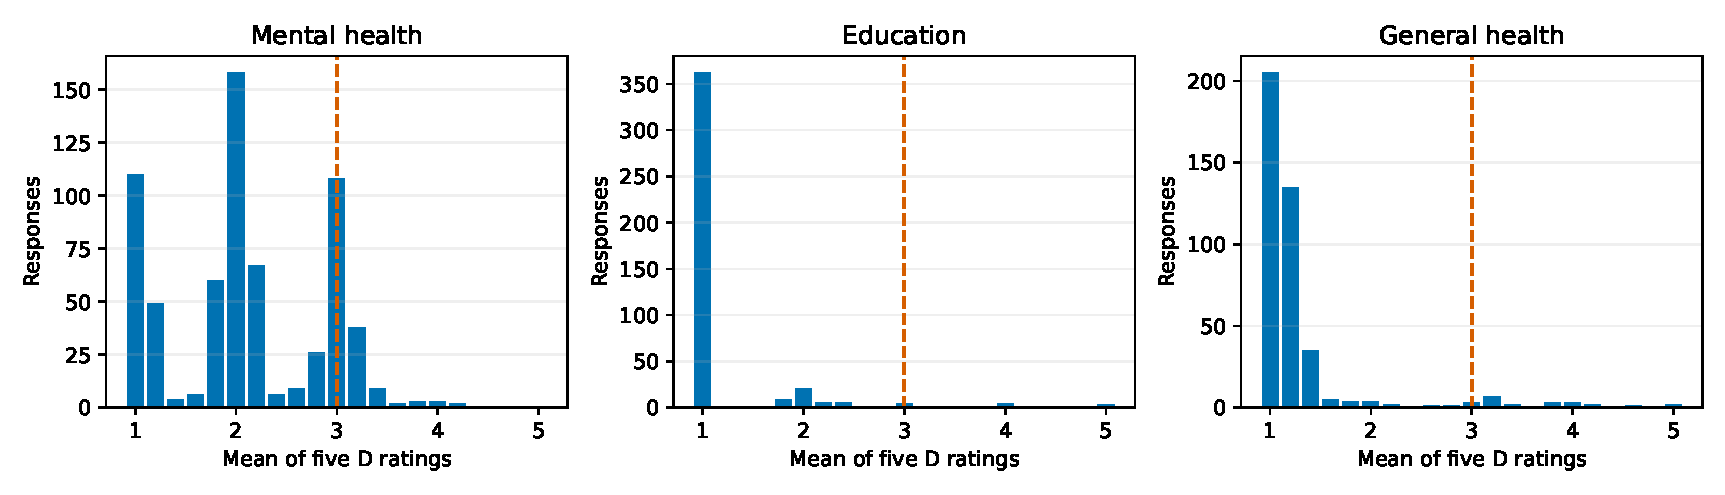
\includegraphics[width=\linewidth]{figures/d_mean_distributions.pdf}
\caption{Descriptive distributions of five-rater D means. Dashed lines mark the original mean-$D\geq3$ cutoff. Counts, not fitted densities, show the concentration of values; panels use separate count scales.}
\Description{Bar charts show D means from one to five in each domain, with a dashed cutoff at three. Mental-health means include many observations at the cutoff; education and general-health means are mostly below it.}
\end{figure}

\section{Transfer and Complementarity Details}\label{app:transfer}
These are exploratory descriptive comparisons; sparse education D and general-health OA cells do not support confident policy rankings. All domain budget curves remain available here, while the main summary figure shows paired contrasts. Fusion and complementarity were added after the initial analysis and did not replace the original primary comparisons.
For context, oracle recall is $R^*=\min(1,k/P)$ and prevalence-relative lift is $(T/k)/(P/n)$. The achieved fraction of oracle recall is $(T/P)/R^*$. When $0<k\leq P$, this equals precision $T/k$ algebraically, not coincidentally; these quantities are not independent evidence. The oracle uses unavailable labels and is not an implementable policy.
\begin{table}[t]
\centering\small
\caption{Descriptive capacity context for high-H at 20\%. Recall and oracle quantities are percentages; lift is precision divided by prevalence. Oracle is an unavailable-label upper bound, not an implementable policy.}
\label{tab:oracle_context}
\begin{tabular}{llrrrr}
\toprule
Domain & Criterion & Recall & Oracle recall & Fraction of oracle & Lift \\
\midrule
Mental health & $\overline D\geq3$ & 25.5 & 80.0 & 31.8 & 1.27 \\
 & $\overline F<4$ & 18.9 & 100.0 & 18.9 & 0.95 \\
 & $\overline{\mathrm{OA}}<4$ & 23.3 & 99.2 & 23.5 & 1.17 \\
Education & $\overline D\geq3$ & 58.3 & 100.0 & 58.3 & 2.92 \\
 & $\overline F<4$ & 40.0 & 100.0 & 40.0 & 2.00 \\
 & $\overline{\mathrm{OA}}<4$ & 50.0 & 100.0 & 50.0 & 2.50 \\
General health & $\overline D\geq3$ & 43.5 & 100.0 & 43.5 & 2.17 \\
 & $\overline F<4$ & 20.8 & 69.2 & 30.1 & 1.04 \\
 & $\overline{\mathrm{OA}}<4$ & 33.3 & 100.0 & 33.3 & 1.67 \\
\bottomrule
\end{tabular}
\end{table}

\begin{table}[t]
\centering\small
\caption{Post-review exploratory complementarity at the original 20\% budget. H-only/marker-only/both are concern counts in the two selected sets; their union exceeds the budget and is not a policy. Fusion is an exact-budget equal-weight midrank policy. Differences are recall percentage points with exploratory pointwise 95\% intervals; education $D$ and general-health OA remain sparse.}
\label{tab:complementarity}
\begin{tabular}{llrrrrr}
\toprule
Domain & Criterion & H only & M only & Both & Fusion/$P$ & $\Delta R$ [95\%] \\
\midrule
Mental health & $\overline D\geq3$ & 20 & 41 & 22 & 61/165 & -1.2 [-7.9, +5.0] \\
 & $\overline F<4$ & 13 & 17 & 5 & 25/95 & +3.2 [-6.6, +10.6] \\
 & $\overline{\mathrm{OA}}<4$ & 19 & 21 & 12 & 39/133 & +4.5 [-2.3, +11.5] \\
Education & $\overline D\geq3$ & 1 & 3 & 6 & 9/12 & +0.0 [-33.3, +36.4] \\
 & $\overline F<4$ & 10 & 1 & 0 & 3/25 & +8.0 [+0.0, +23.1] \\
 & $\overline{\mathrm{OA}}<4$ & 9 & 3 & 0 & 3/18 & +0.0 [-16.7, +25.0] \\
General health & $\overline D\geq3$ & 0 & 11 & 10 & 17/23 & -17.4 [-38.5, +0.0] \\
 & $\overline F<4$ & 10 & 17 & 15 & 31/120 & -0.8 [-7.1, +5.4] \\
 & $\overline{\mathrm{OA}}<4$ & 0 & 6 & 3 & 7/9 & -22.2 [-60.0, +0.0] \\
\bottomrule
\end{tabular}
\end{table}

\begin{table}[t]
\centering\small
\caption{Mental-health workload for 80\% recall of $\overline D\geq3$. Random workload is an expected order statistic, not a guaranteed stopping point. Intervals are exploratory pointwise 95\%; paired differences are reported in the text.}
\label{tab:workload}
\begin{tabular}{llr}
\toprule
Domain & Policy & Batch percentage [95\% CI] \\
\midrule
Mental health & HumT & 70.8 [64.1, 77.3] \\
 & Length & 66.1 [58.6, 73.8] \\
 & Markers & 63.3 [52.9, 71.1] \\
 & Random (expected) & 79.6 [79.6, 80.1] \\
\bottomrule
\end{tabular}
\end{table}

\begin{table}[t]
\centering\small
\caption{Education and general-health retrospective workload for 80\% recall of $\overline D\geq3$. Intervals are exploratory pointwise 95\%; education has only seven concern-bearing prompts.}
\label{tab:workload_transfer}
\begin{tabular}{llr}
\toprule
Domain & Policy & Batch percentage [95\% CI] \\
\midrule
Education & HumT & 37.6 [9.2, 83.7] \\
 & Length & 67.7 [29.0, 96.4] \\
 & Markers & 23.9 [9.9, 38.1] \\
 & Random (expected) & 77.1 [66.8, 80.2] \\
General health & HumT & 46.3 [28.5, 61.4] \\
 & Length & 83.4 [70.5, 93.0] \\
 & Markers & 15.2 [9.8, 32.9] \\
 & Random (expected) & 79.4 [75.2, 80.2] \\
\bottomrule
\end{tabular}
\end{table}

\begin{figure}[t]
\centering
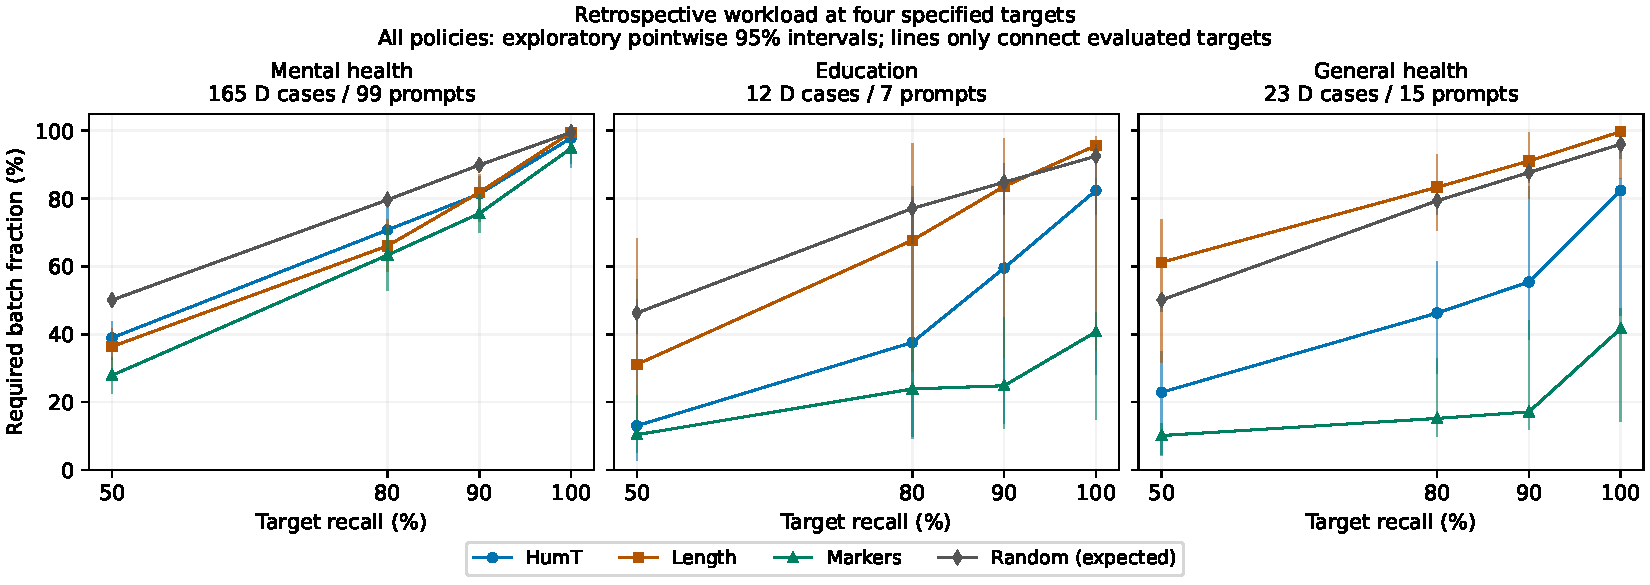
\includegraphics[width=\linewidth]{figures/workload_targets.pdf}
\caption{Retrospective workload for all four specified broad-$D$ recall targets, with exploratory pointwise 95\% intervals for every policy. Lines connect evaluated targets only; random values are expected order statistics. Sparse education support limits precision. Targets are descriptive, not stakeholder-validated service requirements or deployable stopping rules.}
\Description{Three panels show batch percentages for 50, 80, 90 and 100 percent D recall in each domain. HumT, length, markers and random have uncertainty bars; workload rises with target recall.}
\label{fig:workloadtargets}
\end{figure}
\begin{figure}[t]
\centering
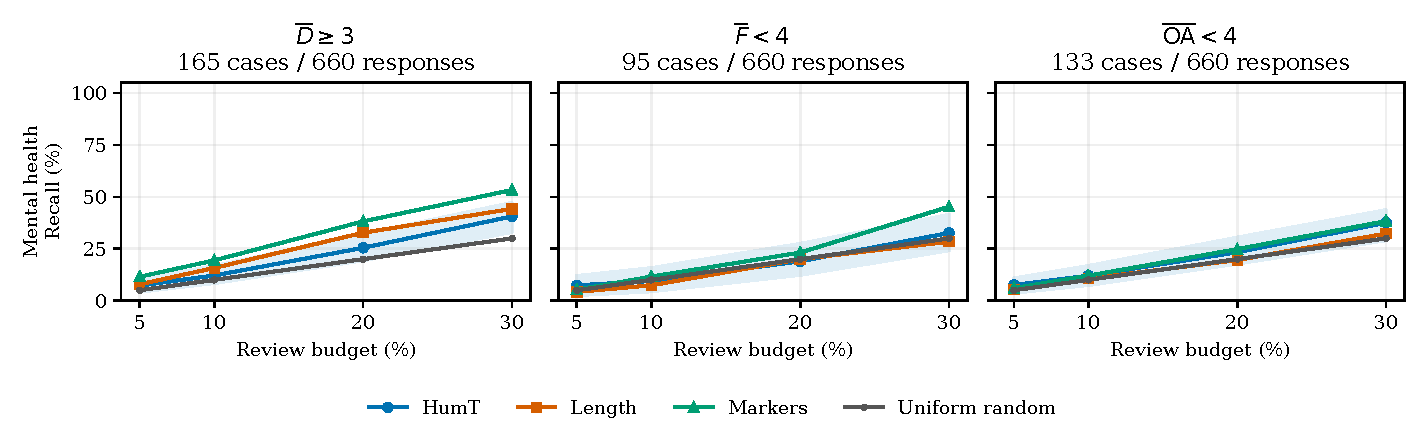
\includegraphics[width=\linewidth]{figures/mental_health_budgets.pdf}
\caption{Original mental-health budget curves. Shading shows only HumT's exploratory pointwise 95\% intervals, not uncertainty-free baselines. Figure~\ref{fig:paired} provides paired policy-difference intervals; complete marginal intervals are retained in the computational record.}
\Description{Three mental-health panels compare HumT, length, markers, and analytical random recall across four budgets and three criteria.}
\label{fig:budgets}
\end{figure}
\begin{figure}[t]
\centering
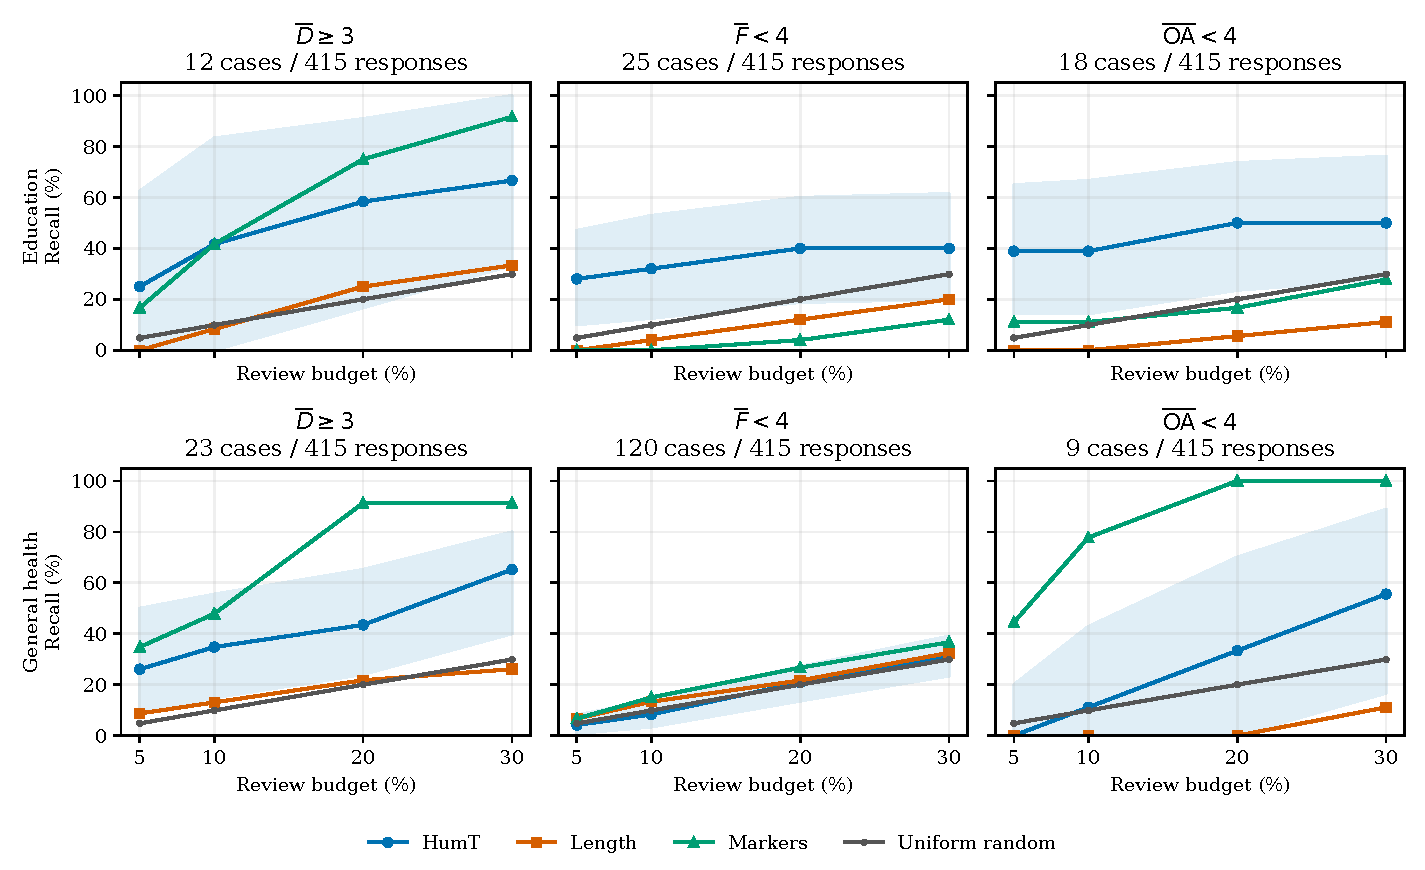
\includegraphics[width=\linewidth]{figures/transfer_budgets.pdf}
\caption{Education and general-health budget curves. Shading shows HumT's exploratory pointwise 95\% intervals, not simultaneous bands; random values are analytical expectations. Sparse cells and different prevalences constrain interpretation.}
\Description{Six panels retain recall curves for education and general health under all three criteria and four budgets. Education D and general-health OA have wide uncertainty despite some high observed recall values.}
\end{figure}

\section{Complete Policy Comparisons}\label{app:complete}
The following tables retain every D, fit, and OA policy cell at the reference fraction, including unfavorable and sparse results. Tables~\ref{tab:full_mental_health}--\ref{tab:full_health} use the original full-domain batches and add fixed fusion. Tables~\ref{tab:held_mental_health}--\ref{tab:held_health} re-evaluate all seven policies in identical held-out batches. Their capacities and bootstrap procedures differ; the two table families must not be combined into an apparent matched-budget comparison. Random counts are expectations, so they can be fractional. The record retains all four budgets, selected and missed counts, precision, recall, unselected prevalence, and paired differences from random. Only the reference fraction has intervals for the trained amendment.
\begin{table}[t]
\centering\small
\caption{Mental health: all full-batch policies and criteria at 20\% (132 slots). Precision and recall are percentages; $P$ denotes cases. Intervals are exploratory pointwise 95\%; random counts are analytical expectations. Fusion is the first post-review addition. Education $D$ and general-health OA are sparse.}
\label{tab:full_mental_health}
\begin{tabular}{llrrrr}
\toprule
Criterion & Policy & Caught/$P$ & Prec. & Recall [95\% CI] & Missed \\
\midrule
$\overline D\geq3$ & HumT & 42/165 & 31.8 & 25.5 [19.2, 32.1] & 123 \\
 & Length & 54/165 & 40.9 & 32.7 [26.9, 37.9] & 111 \\
 & Markers & 63/165 & 47.7 & 38.2 [31.7, 45.8] & 102 \\
 & Rank fusion & 61/165 & 46.2 & 37.0 [30.5, 43.5] & 104 \\
 & Random (expected) & 33/165 & 25.0 & 20.0 [20.0, 20.0] & 132 \\
$\overline F<4$ & HumT & 18/95 & 13.6 & 18.9 [12.2, 27.6] & 77 \\
 & Length & 19/95 & 14.4 & 20.0 [12.7, 27.0] & 76 \\
 & Markers & 22/95 & 16.7 & 23.2 [15.6, 32.1] & 73 \\
 & Rank fusion & 25/95 & 18.9 & 26.3 [17.0, 33.8] & 70 \\
 & Random (expected) & 19/95 & 14.4 & 20.0 [20.0, 20.0] & 76 \\
$\overline{\mathrm{OA}}<4$ & HumT & 31/133 & 23.5 & 23.3 [17.6, 30.6] & 102 \\
 & Length & 26/133 & 19.7 & 19.5 [15.0, 26.6] & 107 \\
 & Markers & 33/133 & 25.0 & 24.8 [18.3, 31.2] & 100 \\
 & Rank fusion & 39/133 & 29.5 & 29.3 [22.1, 36.1] & 94 \\
 & Random (expected) & 26.6/133 & 20.2 & 20.0 [20.0, 20.0] & 106.4 \\
\bottomrule
\end{tabular}
\end{table}

\begin{table}[t]
\centering\small
\caption{Education: all full-batch policies and criteria at 20\% (83 slots). Precision and recall are percentages; $P$ denotes cases. Intervals are exploratory pointwise 95\%; random counts are analytical expectations. Fusion is the first post-review addition. Education $D$ and general-health OA are sparse.}
\label{tab:full_education}
\begin{tabular}{llrrrr}
\toprule
Criterion & Policy & Caught/$P$ & Prec. & Recall [95\% CI] & Missed \\
\midrule
$\overline D\geq3$ & HumT & 7/12 & 8.4 & 58.3 [16.7, 90.9] & 5 \\
 & Length & 3/12 & 3.6 & 25.0 [0.0, 60.0] & 9 \\
 & Markers & 9/12 & 10.8 & 75.0 [38.5, 100.0] & 3 \\
 & Rank fusion & 9/12 & 10.8 & 75.0 [37.4, 100.0] & 3 \\
 & Random (expected) & 2.4/12 & 2.9 & 20.0 [19.9, 20.0] & 9.6 \\
$\overline F<4$ & HumT & 10/25 & 12.0 & 40.0 [18.8, 60.0] & 15 \\
 & Length & 3/25 & 3.6 & 12.0 [0.0, 31.2] & 22 \\
 & Markers & 1/25 & 1.2 & 4.0 [0.0, 12.5] & 24 \\
 & Rank fusion & 3/25 & 3.6 & 12.0 [0.0, 26.7] & 22 \\
 & Random (expected) & 5/25 & 6.0 & 20.0 [19.9, 20.0] & 20 \\
$\overline{\mathrm{OA}}<4$ & HumT & 9/18 & 10.8 & 50.0 [23.5, 73.7] & 9 \\
 & Length & 1/18 & 1.2 & 5.6 [0.0, 22.2] & 17 \\
 & Markers & 3/18 & 3.6 & 16.7 [0.0, 40.0] & 15 \\
 & Rank fusion & 3/18 & 3.6 & 16.7 [0.0, 40.0] & 15 \\
 & Random (expected) & 3.6/18 & 4.3 & 20.0 [19.9, 20.0] & 14.4 \\
\bottomrule
\end{tabular}
\end{table}

\begin{table}[t]
\centering\small
\caption{General health: all full-batch policies and criteria at 20\% (83 slots). Precision and recall are percentages; $P$ denotes cases. Intervals are exploratory pointwise 95\%; random counts are analytical expectations. Fusion is the first post-review addition. Education $D$ and general-health OA are sparse.}
\label{tab:full_health}
\begin{tabular}{llrrrr}
\toprule
Criterion & Policy & Caught/$P$ & Prec. & Recall [95\% CI] & Missed \\
\midrule
$\overline D\geq3$ & HumT & 10/23 & 12.0 & 43.5 [24.0, 65.2] & 13 \\
 & Length & 5/23 & 6.0 & 21.7 [5.4, 40.7] & 18 \\
 & Markers & 21/23 & 25.3 & 91.3 [75.9, 100.0] & 2 \\
 & Rank fusion & 17/23 & 20.5 & 73.9 [52.0, 95.0] & 6 \\
 & Random (expected) & 4.6/23 & 5.5 & 20.0 [19.8, 20.0] & 18.4 \\
$\overline F<4$ & HumT & 25/120 & 30.1 & 20.8 [13.6, 27.2] & 95 \\
 & Length & 26/120 & 31.3 & 21.7 [16.5, 27.9] & 94 \\
 & Markers & 32/120 & 38.6 & 26.7 [18.0, 33.8] & 88 \\
 & Rank fusion & 31/120 & 37.3 & 25.8 [16.8, 32.3] & 89 \\
 & Random (expected) & 24/120 & 28.9 & 20.0 [19.8, 20.0] & 96 \\
$\overline{\mathrm{OA}}<4$ & HumT & 3/9 & 3.6 & 33.3 [0.0, 70.1] & 6 \\
 & Length & 0/9 & 0.0 & 0.0 [0.0, 20.0] & 9 \\
 & Markers & 9/9 & 10.8 & 100.0 [82.4, 100.0] & 0 \\
 & Rank fusion & 7/9 & 8.4 & 77.8 [40.0, 100.0] & 2 \\
 & Random (expected) & 1.8/9 & 2.2 & 20.0 [19.8, 20.0] & 7.2 \\
\bottomrule
\end{tabular}
\end{table}

\begin{table}[t]
\centering\small
\caption{Mental health: every policy in the same five held-out batches, with 130 total slots at the 20\% reference fraction. LR models use training labels; other rules are label-free. Precision and recall are percentages. Intervals are exploratory pointwise 95\% from paired refits, conditional on the fixed partition; sparse cells remain descriptive. Random counts are expectations. Do not compare these directly with the different full-batch capacities.}
\label{tab:held_mental_health}
\begin{tabular}{llrrrr}
\toprule
Criterion & Policy & Caught/$P$ & Prec. & Recall [95\% CI] & Missed \\
\midrule
$\overline D\geq3$ & HumT & 42/165 & 32.3 & 25.5 [19.9, 31.7] & 123 \\
 & Length & 49/165 & 37.7 & 29.7 [25.5, 37.0] & 116 \\
 & Markers & 63/165 & 48.5 & 38.2 [31.1, 45.9] & 102 \\
 & Rank fusion & 61/165 & 46.9 & 37.0 [30.3, 42.6] & 104 \\
 & LR: markers + length & 70/165 & 53.8 & 42.4 [34.2, 48.2] & 95 \\
 & LR: + HumT & 66/165 & 50.8 & 40.0 [32.4, 46.9] & 99 \\
 & Random (expected) & 32.50/165 & 25.0 & 19.7 [19.7, 19.7] & 132.50 \\
$\overline F<4$ & HumT & 18/95 & 13.8 & 18.9 [12.5, 28.0] & 77 \\
 & Length & 18/95 & 13.8 & 18.9 [12.0, 26.3] & 77 \\
 & Markers & 24/95 & 18.5 & 25.3 [16.7, 35.0] & 71 \\
 & Rank fusion & 25/95 & 19.2 & 26.3 [17.3, 35.4] & 70 \\
 & LR: markers + length & 32/95 & 24.6 & 33.7 [22.1, 44.2] & 63 \\
 & LR: + HumT & 33/95 & 25.4 & 34.7 [20.2, 43.0] & 62 \\
 & Random (expected) & 18.71/95 & 14.4 & 19.7 [19.7, 19.7] & 76.29 \\
$\overline{\mathrm{OA}}<4$ & HumT & 30/133 & 23.1 & 22.6 [16.1, 29.1] & 103 \\
 & Length & 29/133 & 22.3 & 21.8 [15.2, 27.5] & 104 \\
 & Markers & 29/133 & 22.3 & 21.8 [15.9, 29.3] & 104 \\
 & Rank fusion & 37/133 & 28.5 & 27.8 [21.1, 34.2] & 96 \\
 & LR: markers + length & 26/133 & 20.0 & 19.5 [14.5, 30.2] & 107 \\
 & LR: + HumT & 30/133 & 23.1 & 22.6 [15.1, 31.9] & 103 \\
 & Random (expected) & 26.20/133 & 20.2 & 19.7 [19.7, 19.7] & 106.80 \\
\bottomrule
\end{tabular}
\end{table}

\begin{table}[t]
\centering\small
\caption{Education: every policy in the same five held-out batches, with 80 total slots at the 20\% reference fraction. LR models use training labels; other rules are label-free. Precision and recall are percentages. Intervals are exploratory pointwise 95\% from paired refits, conditional on the fixed partition; sparse cells remain descriptive. Random counts are expectations. Do not compare these directly with the different full-batch capacities.}
\label{tab:held_education}
\begin{tabular}{llrrrr}
\toprule
Criterion & Policy & Caught/$P$ & Prec. & Recall [95\% CI] & Missed \\
\midrule
$\overline D\geq3$ & HumT & 8/12 & 10.0 & 66.7 [28.6, 88.9] & 4 \\
 & Length & 3/12 & 3.8 & 25.0 [0.0, 55.7] & 9 \\
 & Markers & 8/12 & 10.0 & 66.7 [36.4, 100.0] & 4 \\
 & Rank fusion & 10/12 & 12.5 & 83.3 [39.8, 100.0] & 2 \\
 & LR: markers + length & 7/12 & 8.8 & 58.3 [14.3, 100.0] & 5 \\
 & LR: + HumT & 8/12 & 10.0 & 66.7 [9.0, 86.7] & 4 \\
 & Random (expected) & 2.33/12 & 2.9 & 19.4 [19.1, 19.8] & 9.67 \\
$\overline F<4$ & HumT & 9/25 & 11.2 & 36.0 [18.2, 57.1] & 16 \\
 & Length & 3/25 & 3.8 & 12.0 [0.0, 27.3] & 22 \\
 & Markers & 1/25 & 1.2 & 4.0 [0.0, 16.7] & 24 \\
 & Rank fusion & 3/25 & 3.8 & 12.0 [0.0, 26.1] & 22 \\
 & LR: markers + length & 13/25 & 16.2 & 52.0 [6.7, 73.9] & 12 \\
 & LR: + HumT & 13/25 & 16.2 & 52.0 [7.7, 73.1] & 12 \\
 & Random (expected) & 4.79/25 & 6.0 & 19.1 [19.0, 19.3] & 20.21 \\
$\overline{\mathrm{OA}}<4$ & HumT & 8/18 & 10.0 & 44.4 [21.4, 71.4] & 10 \\
 & Length & 1/18 & 1.2 & 5.6 [0.0, 23.1] & 17 \\
 & Markers & 3/18 & 3.8 & 16.7 [0.0, 45.0] & 15 \\
 & Rank fusion & 4/18 & 5.0 & 22.2 [0.0, 41.7] & 14 \\
 & LR: markers + length & 12/18 & 15.0 & 66.7 [0.0, 91.7] & 6 \\
 & LR: + HumT & 12/18 & 15.0 & 66.7 [0.0, 90.9] & 6 \\
 & Random (expected) & 3.44/18 & 4.3 & 19.1 [19.0, 19.2] & 14.56 \\
\bottomrule
\end{tabular}
\end{table}

\begin{table}[t]
\centering\small
\caption{General health: every policy in the same five held-out batches, with 80 total slots at the 20\% reference fraction. LR models use training labels; other rules are label-free. Precision and recall are percentages. Intervals are exploratory pointwise 95\% from paired refits, conditional on the fixed partition; sparse cells remain descriptive. Random counts are expectations. Do not compare these directly with the different full-batch capacities.}
\label{tab:held_health}
\begin{tabular}{llrrrr}
\toprule
Criterion & Policy & Caught/$P$ & Prec. & Recall [95\% CI] & Missed \\
\midrule
$\overline D\geq3$ & HumT & 10/23 & 12.5 & 43.5 [26.7, 66.7] & 13 \\
 & Length & 5/23 & 6.2 & 21.7 [6.2, 40.0] & 18 \\
 & Markers & 21/23 & 26.2 & 91.3 [60.9, 100.0] & 2 \\
 & Rank fusion & 18/23 & 22.5 & 78.3 [52.0, 92.3] & 5 \\
 & LR: markers + length & 21/23 & 26.2 & 91.3 [57.1, 100.0] & 2 \\
 & LR: + HumT & 21/23 & 26.2 & 91.3 [54.2, 96.0] & 2 \\
 & Random (expected) & 4.44/23 & 5.6 & 19.3 [19.0, 19.6] & 18.56 \\
$\overline F<4$ & HumT & 23/120 & 28.7 & 19.2 [12.7, 26.3] & 97 \\
 & Length & 27/120 & 33.8 & 22.5 [16.8, 29.2] & 93 \\
 & Markers & 32/120 & 40.0 & 26.7 [16.4, 32.3] & 88 \\
 & Rank fusion & 28/120 & 35.0 & 23.3 [15.8, 30.8] & 92 \\
 & LR: markers + length & 29/120 & 36.2 & 24.2 [12.7, 31.8] & 91 \\
 & LR: + HumT & 30/120 & 37.5 & 25.0 [14.4, 31.5] & 90 \\
 & Random (expected) & 23.14/120 & 28.9 & 19.3 [19.1, 19.5] & 96.86 \\
$\overline{\mathrm{OA}}<4$ & HumT & 3/9 & 3.8 & 33.3 [0.0, 72.7] & 6 \\
 & Length & 0/9 & 0.0 & 0.0 [0.0, 20.1] & 9 \\
 & Markers & 9/9 & 11.2 & 100.0 [60.0, 100.0] & 0 \\
 & Rank fusion & 7/9 & 8.8 & 77.8 [33.3, 100.0] & 2 \\
 & LR: markers + length & 8/9 & 10.0 & 88.9 [50.0, 100.0] & 1 \\
 & LR: + HumT & 8/9 & 10.0 & 88.9 [50.0, 100.0] & 1 \\
 & Random (expected) & 1.73/9 & 2.2 & 19.3 [19.0, 19.6] & 7.27 \\
\bottomrule
\end{tabular}
\end{table}

\begin{table}[htbp]
\centering\small
\caption{Conditional-lift sensitivity across ten additional pre-specified prompt partitions. Ranges are descriptive, not confidence intervals or independent replication. Finite draws count defined paired differences in the original-partition 2,000-draw bootstrap; $\dagger$ marks sparse cells. All seed-level results are retained, not just a favorable partition.}
\label{tab:split_sensitivity}
\begin{tabular}{llrrr}
\toprule
Domain & Criterion & Positive prompts & Finite draws & Split range, pp \\
\midrule
Mental health & $\overline D\geq3$ & 99 & 2000 & [-3.0, +1.2] \\
 & $\overline F<4$ & 77 & 2000 & [-5.3, +1.1] \\
 & $\overline{\mathrm{OA}}<4$ & 111 & 2000 & [-1.5, +4.5] \\
Education & $\overline D\geq3$$^{\dagger}$ & 7 & 1998 & [-8.3, +0.0] \\
 & $\overline F<4$ & 17 & 2000 & [-4.0, +4.0] \\
 & $\overline{\mathrm{OA}}<4$ & 10 & 2000 & [+0.0, +0.0] \\
General health & $\overline D\geq3$ & 15 & 2000 & [-8.7, +4.3] \\
 & $\overline F<4$ & 69 & 2000 & [-3.3, +1.7] \\
 & $\overline{\mathrm{OA}}<4$$^{\dagger}$ & 7 & 1998 & [+0.0, +0.0] \\
\bottomrule
\end{tabular}
\end{table}


Each mental-health model uses 528 training responses (2,640 underlying criterion ratings); education uses 331--334 (1,655--1,670 ratings); general health uses 331--333 (1,655--1,665 ratings). Training sets overlap across fits and these are not additive acquisition costs. No point-estimate fit needed the single-class fallback. Across all criteria and models, it occurred in 68/2,000 education draws and 50/2,000 general-health draws (154 and 116 model fits), and no mental-health draw. Undefined paired recall differences occur in two education-D and two general-health-OA draws; those cells retain 1,998 finite draws. All other conditional-lift cells retain 2,000. These counts belong to the new refitted bootstrap, not the original intervals below.

\section{Common-Queue Coverage Details}\label{app:queue}
\begin{table}[t]
\centering\small
\caption{Where review slots go in the common full-domain queues: 132 mental-health slots and 83 in each other domain. Category counts are projections of one queue, not independent quotas. Selection is label-free and identical across D/F/OA endpoints; natural/adversarial prompts are unmatched.}
\label{tab:common_queue_slots}
\begin{tabular}{llrrr}
\toprule
Domain & Condition & Responses & HumT slots & Marker slots \\
\midrule
Mental health & Natural & 300 & 78 & 63 \\
 & Adversarial & 360 & 54 & 69 \\
Education & Natural & 268 & 41 & 15 \\
 & Adversarial & 147 & 42 & 68 \\
General health & Natural & 265 & 27 & 12 \\
 & Adversarial & 150 & 56 & 71 \\
\bottomrule
\end{tabular}
\end{table}

\begin{table}[t]
\centering\small
\caption{All condition-by-criterion results projected from common queues. Cases/prompts gives concern responses and supporting prompts. H and M denote HumT and markers; paired differences are exploratory pointwise, not simultaneous. $\dagger$ marks fewer than ten positive or negative supporting prompts; a zero-concern group has undefined recall, not perfect or zero coverage. All policies and model/scenario categories remain in the computational record.}
\label{tab:common_queue_conditions}
\begin{tabular}{lllrrr}
\toprule
Domain / target & Condition & Cases/prompts & H caught & M caught & H--M recall, pp [95\%] \\
\midrule
Mental health / D & Natural & 84/49 & 21 & 30 & -10.7 [-24.4, +2.2] \\
 & Adversarial & 81/50 & 21 & 33 & -14.8 [-28.4, -2.5] \\
Mental health / Fit & Natural & 47/40 & 11 & 11 & +0.0 [-15.6, +16.3] \\
 & Adversarial & 48/37 & 7 & 11 & -8.3 [-25.0, +9.3] \\
Mental health / OA & Natural & 69/57 & 22 & 18 & +5.8 [-5.9, +21.2] \\
 & Adversarial & 64/54 & 9 & 15 & -9.4 [-22.7, +3.6] \\
Education / D & Natural$^{\dagger}$ & 0/0 & 0 & 0 & Undefined \\
 & Adversarial$^{\dagger}$ & 12/7 & 7 & 9 & -16.7 [-50.0, +16.7] \\
Education / Fit & Natural$^{\dagger}$ & 9/8 & 1 & 0 & +11.1 [+0.0, +40.0] \\
 & Adversarial$^{\dagger}$ & 16/9 & 9 & 1 & +50.0 [+22.2, +77.8] \\
Education / OA & Natural$^{\dagger}$ & 0/0 & 0 & 0 & Undefined \\
 & Adversarial & 18/10 & 9 & 3 & +33.3 [-7.7, +71.4] \\
General health / D & Natural$^{\dagger}$ & 3/3 & 1 & 2 & -33.3 [-100.0, +0.0] \\
 & Adversarial & 20/12 & 9 & 19 & -50.0 [-66.7, -26.7] \\
General health / Fit & Natural & 74/46 & 8 & 4 & +5.4 [-1.3, +13.0] \\
 & Adversarial & 46/23 & 17 & 28 & -23.9 [-41.2, -4.5] \\
General health / OA & Natural$^{\dagger}$ & 0/0 & 0 & 0 & Undefined \\
 & Adversarial$^{\dagger}$ & 9/7 & 3 & 9 & -66.7 [-100.0, -28.5] \\
\bottomrule
\end{tabular}
\end{table}

This table projects fixed selections onto the two recorded prompt conditions. It does not recreate the earlier procedure that allocated 20\% within each subgroup. The full record contains 525 category/criterion/policy cells over condition, model, and scenario partitions, including zero-concern groups. Each partition's selected and caught totals reconstruct the original full-domain results. Group-versus-complement recall contrasts are undefined when either side has no concern cases; these draws retain explicit finite counts rather than substituted zeros. Random precision in the category table is the ratio of expected caught cases to expected slots, not the expectation of a random ratio. No new demographic attributes or cue-category annotations were inferred.

\section{Criterion and Text-Provenance Sensitivity}\label{app:sensitivity}
Mental-health metadata and HumT scores are embedded without historical scorer-input strings. Transfer-domain prompt IDs are reconstructed from text and model attribution from HumT source files. Replaying the join reproduces every score and join tier. Of 830 export/rated pairs, 771 are byte-identical; 56 education and three general-health pairs differ after normalization (52 prefix and seven fuzzy joins). These are not merely cosmetic differences. Baselines use annotated response text, and exports alone do not authenticate historical scorer calls. All rows and original scores are preserved.

At the stricter mean-$D\geq4$ threshold, high-H selects zero of five mental-health cases, three of eight education cases, and two of eight general-health cases at 20\%. These concerns occur in only four, five, and six prompt clusters. These sparse stronger-anchor results are not precise deployment estimates, and thresholds are not interchangeable choices from which to select a favorable result.

Requiring at least three of five ratings to meet $D\geq3$ yields high-H captures of 48/200, 12/22, and 11/24 across the three domains. Requiring all five yields 39/150, 7/12, and 6/17. Agreement does not validate the normative criterion. Only six mental-health, four education, and six general-health responses satisfy all three primary criteria. The record retains all eight intersections and continuous relationships: cut points and prevalence can explain low overlap without establishing normative disagreement. Trained models were not refitted for these threshold variants.

Recomputing length and markers from HumT export strings on unchanged full batches leaves their selected concern counts unchanged at 20\% for all three criteria in both transfer domains; fusion counts are also unchanged. This does not establish identical selected identities or correct historical scorer calls. A separate reconstruction checked all 48 previously reported subset operating points using byte equality explicitly, rather than assuming the stored join tier implies identical text.

\begin{table}[t]
\centering\small
\caption{Available export/rated-text composition. Counts are criterion cases, not harms. Identical strings do not authenticate historical scorer calls; excluded rows change the evaluation population.}
\label{tab:provenance_composition}
\begin{tabular}{llrrrr}
\toprule
Domain & Text pair & $n$ & $D$ cases & $F$ cases & OA cases \\
\midrule
Education & Identical & 359 & 12 & 23 & 18 \\
Education & Different & 56 & 0 & 2 & 0 \\
General health & Identical & 412 & 23 & 120 & 9 \\
General health & Different & 3 & 0 & 0 & 0 \\
\bottomrule
\end{tabular}
\end{table}

The available scorer code truncates its input to 300 characters. 830/830 recorded \texttt{text\_trunc} fields match their export's first 300 characters, but only 369/415 education and 414/415 general-health fields match the rated text's first 300 characters. Thus 12 of the 59 differing full-text pairs retain the same recorded prefix and 47 do not. This is evidence about available export preprocessing, not authentication that the available code/version produced the historical score. No score is replaced.


The 56 differing education pairs contain no broad-$D$ or OA cases and two fit cases; the three differing general-health pairs contain none of these criterion cases. Nevertheless, their presence can affect competition for review slots. Keeping only byte-identical pairs and retaining the absolute capacity of 83 captures seven of 12 education broad-$D$ cases and ten of 23 general-health cases. At 20\% of the smaller batches, 71 and 82 slots capture six and ten cases. Full condition/model/scenario composition and all four ranked-policy operating points are retained in the computational record. The subset analysis is descriptive, not a paired causal estimate of join error, and does not authenticate the historical scorer invocation. Mental-health scores remain embedded without a separate scorer-input string.

\section{Assessment Follow-up: Complete Sensitivity}\label{app:assessment}
R1, R2 and R3 correspond to archive assessor streams A, B and C, respectively, not the original study's rater groups. Observed R1/R2 agreement is reported before majority resolution. R3 saw only disputed cases and used note v1.1; selective resolution cannot establish reliability on undisputed responses or identify the effect of changing the capability note. The documented version change distinguishes assumptions about monitoring and external actions from verified capabilities, rather than proving what the original model could do. Missing tool logs are not proof of absent capabilities.

\begin{table}[htbp]
\centering\small
\caption{Assessor and target sensitivity at the same 132 slots. $\Delta R$ is HumT minus normalized-marker recall in percentage points. Pointwise intervals use 2,000 paired prompt-cluster draws with re-ranking. Dashes mean intervals were not estimated, not zero uncertainty. Person and capability-note version are confounded; resolved judgments do not create a third full-corpus rating stream.}
\label{tab:annotation_sensitivity}
\begin{tabular}{lrrrrr}
\toprule
Target & $P$ & H caught & M caught & $\Delta R$ & 95\% interval \\
\midrule
R1 alone & 29 & 10 & 16 & -20.7 & [-47.6, +9.3] \\
R2 alone & 19 & 6 & 10 & -21.1 & [-50.0, +9.1] \\
Resolved & 19 & 6 & 12 & -31.6 & [-66.7, +4.3] \\
R1/R2 union & 31 & 10 & 16 & -19.4 & -- \\
R1/R2 intersection & 17 & 6 & 10 & -23.5 & -- \\
R1 rating 3 & 15 & 5 & 8 & -20.0 & -- \\
R2 rating 3 & 7 & 1 & 4 & -42.9 & -- \\
\bottomrule
\end{tabular}
\end{table}

\begin{table}[t]
\centering\small
\caption{All four specified budgets under the resolved follow-up target ($P=19$). H, M and L denote HumT, normalized markers and word length. Random values are expected captured counts. The 20\% fraction was already explored, not selected to optimize these new judgments.}
\label{tab:annotation_budgets}
\begin{tabular}{rrrrrr}
\toprule
Budget (\%) & Slots & H caught & M caught & L caught & Random \\
\midrule
5.0 & 33 & 3 & 4 & 0 & 0.95 \\
10.0 & 66 & 4 & 7 & 1 & 1.9 \\
20.0 & 132 & 6 & 12 & 4 & 3.8 \\
30.0 & 198 & 10 & 13 & 5 & 5.7 \\
\bottomrule
\end{tabular}
\end{table}

\begin{table}[t]
\centering\small
\caption{Exact intersections in the 660-response mental-health batch. The new follow-up target is not merely a stricter numerical cutoff of the source ratings. Different criteria, populations and instructions prevent attributing disagreement to any one cause; neither label stream is treated as ground truth for harm.}
\label{tab:annotation_overlap}
\begin{tabular}{lrrrr}
\toprule
Legacy target & Both & Legacy only & Follow-up only & Neither \\
\midrule
$\overline D\geq3$ & 15 & 150 & 4 & 491 \\
$\overline F<4$ & 5 & 90 & 14 & 551 \\
$\overline{\mathrm{OA}}<4$ & 4 & 129 & 15 & 512 \\
\bottomrule
\end{tabular}
\end{table}


The supplied HumT queue shares all 132 selected IDs with the original policy, but its marker and length queues share only 41 and 51, respectively. They operationalize different lexical rankings and are therefore not interchangeable replications of the original policies. The headline comparisons reconstruct the original normalized-marker and word-token definitions from the original corpus; imported-queue results remain a separately labeled sensitivity, and a single imported random draw is not the random expectation. The supplied assessment frame also differs from the original response text in 601 encoding-only cases and from prompt text in 129; IDs and HumT scores agree throughout. We retain original text for original-policy reproducibility and evaluate repaired-text feature rankings separately, without silently replacing source records.

The secondary uncertainty procedure resamples all 220 prompt clusters with replacement, retaining every response to each sampled prompt and re-ranking the resulting batch at 20\% capacity. A draw is paired across policies and label targets, with deterministic occurrence-specific tie keys; the bootstrap seed is 20261010 and the original policy seed remains 20261002. The intervals for R1, R2 and resolved labels use 2,000 effective draws each and are exploratory pointwise percentile intervals without multiplicity adjustment. Exact census differences do not require sampling intervals; this resampling instead asks how the procedure varies over hypothetical batches drawn from the empirical prompt distribution. It neither resamples assessor populations nor estimates judgment error. The new labels are never screening inputs, and no trained-comparator claim is extended to them.

\section{Implementation and Uncertainty Details}\label{app:implementation}
Tokenization uses the Python regular expression \verb|\b\w+\b| after lowercasing. The fixed marker dictionary is: \texttt{i, me, my, mine, myself, we, us, our, ours, ourselves, you, your, yours, yourself, yourselves, hello, hi, hey, thanks, thank, welcome, sorry, please}. The score is the number of matching tokens divided by the token count; an empty response receives zero. Length is that same token count. These deterministic policies require response text but no human outcome labels. HumT uses the recorded source score, with larger values selected first.

The seed is 20261002. Tie keys use the first eight bytes of a SHA256 digest of the seed and stable identifier. Ranking sorts by descending policy score and then ascending tie key. Capacity uses the integer floor, not a score-at-quantile rule, so tied scores cannot inflate the budget. Pooled proportional random allocation uses Hamilton largest remainders with alphabetical domain tie resolution.

Education \Dcrit{} recall has 1,999 finite bootstrap replicates; general-health \OAcrit{} recall has 1,998; the other domain/criterion reference cells have 2,000. Undefined draws are preserved in the record. Primary adjusted intervals use the three-domain family only. No cross-domain, cross-criterion, or model comparison should be interpreted as automatically covered by that adjustment.

The implementation tests exact capacity, score direction, deterministic ties, hand-checkable and tied-score metrics, zero- and all-positive samples, nonfinite scores, clustered resampling, paired comparisons, and exclusion of outcome columns from screening features. Added tests verify prompt separation, training-only scaling, invariance of a held-out fold's predictions to its own labels, single-class fallback, micro-aggregated counts, paired interval reconstruction, and source immutability. Logistic predictions were independently reconstructed with a scikit-learn pipeline. AP and ROC-AUC were checked against scikit-learn 1.8.0. Analysis dependencies include NumPy 2.4.4, pandas 3.0.2, SciPy 1.17.1, and Matplotlib 3.10.8.

The trained models use tolerance $10^{-8}$ and at most 2,000 solver iterations; a convergence warning is an error, not silently accepted. Sorted unique prompt identifiers are permuted with seed 20261002 and divided into five nearly equal prompt-count folds. All policies share stable tie keys within each held-out batch. Bootstrap copies retain the original prompt's fold, with copy-specific deterministic tie keys, preventing the same original prompt from leaking across training and test sets. Alternative partition seeds are 20261003--20261012; no seed is selected based on outcomes. The original-partition models, transformations, fold assignments, out-of-fold scores, and paired bootstrap differences are preserved in the computational record.

\section{Worked Audit-Use Card}\label{app:card}
\begin{description}
\item[Decision and owner.] Proposed evaluator-managed allocation of 132 review slots in a batch of 660 mental-health responses. This is an offline simulation, not an observed institutional workflow.
\item[Measure and rule.] Descending recorded HumT with deterministic seed-based tie resolution. HumT measures human-like tone, not harm probability.
\item[Criterion.] Mean $D\geq3$ under the source rubric; five Group B ratings per response. The trigger includes simulated affect or understanding and does not establish deception experienced by a user.
\item[Coverage.] 42 of 165 criterion cases selected; precision 31.8\%; recall 25.5\% (pointwise 95\% interval 19.2--32.1\%). Random selection catches 33 cases in expectation at the same capacity. The marker comparator catches 63.
\item[Residual concerns.] 123 criterion cases remain among 528 unselected responses. Non-selection is not clearance; responses outside this criterion can contain other concerns.
\item[Uncertainty and limits.] Prompt-cluster bootstrap with 2,000 replicates; dependence on criterion, source population, and a single-turn corpus. No direct evidence of review effectiveness or actual labor savings.
\item[Proposed challenge route.] Permit challenges to the criterion, its application, or allocation separately. Retain disagreements, original ratings, amendments, and reasons. This process remains unevaluated; a low score must not be the sole reason to exclude a concern from consideration.
\end{description}

\section{Relationship to the Companion Study}\label{app:reuse}
The companion PERSONA manuscript studies overall-appropriateness prediction using regression, grouped cross-validation and ablation. The 1,490 responses, original construct judgments and measurement framework are shared with that work. Here the evaluation unit is a fixed-capacity review queue: the additional analyses measure matched-budget coverage, incremental screening value and residual concerns across recorded categories. The follow-up contributes new contextual judgments on the existing 660 mental-health responses, not new responses. The processed files match the available source-supplement snapshot, and checked principal source results agree with the companion manuscript. This documents artifact consistency rather than authenticating a conference upload. Source scores, judgments and prediction results are preserved.

\section{Reading the Supporting Record}
The computational outputs include matched-budget performance; threshold and rater-consensus sensitivity; criterion intersections and continuous relationships; context counts; complete-prompt model comparisons; join and tie sensitivity; and explicitly hypothetical time, cost, and mixture scenarios. The follow-up adds reconstructed labels, pre-resolution agreement, exact-budget comparisons, rater and encoding sensitivity, and a separate exploratory bootstrap. Sparse and undefined cells remain visible rather than being replaced by favorable subsets. Deferred practitioner-session materials are preparation only; they are distinct from the assessment records analyzed here. No organizational-use or practitioner-validation results are claimed.
\end{document}
